%%%%%%%%%%%%%%%%%%%%%%%%%%%%%%%%%%%%%%%%%%%%%%%%%%%%%%%%%%%%%%%%%%%%%%%%%%%%%%%%%%%%%%%%%%%%%%%%%%%%%%%%%%%%%%%%%%%%%%%%%%%%%%%%%%%%%%%%%
\chapter{Addressing Spectrum Efficiency Through Hybrid-Duplex Communications: A Literature Review}
\label{chap:lit_review}
%%%%%%%%%%%%%%%%%%%%%%%%%%%%%%%%%%%%%%%%%%%%%%%%%%%%%%%%%%%%%%%%%%%%%%%%%%%%%%%%%%%%%%%%%%%%%%%%%%%%%%%%%%%%%%%%%%%%%%%%%%%%%%%%%%%%%%%%%
% Section 1 : Introduction
\section{Introduction}

Spectrum scarcity is a major challenge in aeronautical networks. In UAV networks, spectrum scarcity can potentially lead to more sources of interference on the L-band and C-band, which have been allocated for CNPC links. Accordingly, the performance of UAV communications, e.g., reliability, may become degraded \cite{hellaoui2018aerial}. Likewise, spectrum scarcity in MAV networks can also lead to stronger interference experienced in MAV communications. As a consequence, interference-limited MAV communications may not be able to meet reliability and throughput requirements, e.g., bit error rate below $10^{-6}$ \cite{epple2014overview} or data rates of $1.37$ Mbps \cite{zhang2017adaptive}.

As a first step towards addressing spectrum scarcity in aeronautical communications, it is crucial to note the similarities between UAVs and MAVs. In terms of operating altitudes, MAVs can be operated at an altitude between 3 km to 10 km \cite{castillo2018communication} or even beyond 10 km \cite{cao2018airborne}. In contrast, UAV operating altitudes vary between 300 m \cite{motlagh2016low} to beyond 10 km \cite{fotouhi2019survey}. MAVs can also fly at up to 900 km/h \cite{castillo2018communication}, while UAVs can maintain a flight speed between 57.6 km/h to 482 km/h \cite{fotouhi2019survey}. Furthermore, MAVs and UAVs can be designed using multi-rotor or fixed-wing platforms \cite{fotouhi2019survey}.\footnote{The work in this chapter is derived from \cite{ernest2019addressing}, which has been submitted for publication.}

However, several differences are also noted between UAVs and MAVs. First, UAVs can be designed to be extremely lightweight, i.e., weighing less than 100 g \cite{fotouhi2019survey}. UAVs also have limited range, flight time, and supported payload weight when compared to MAVs \cite{fotouhi2019survey}. 

\begin{figure*}[t]
\centering
\subfloat[MAV Network]{\includegraphics [width=0.49\columnwidth]{chap2_fig/multi_MAV_network_example.eps} 
\label{fig:lit_review_multi_MAV_network_example}}
\hfil
\subfloat[UAV Network]{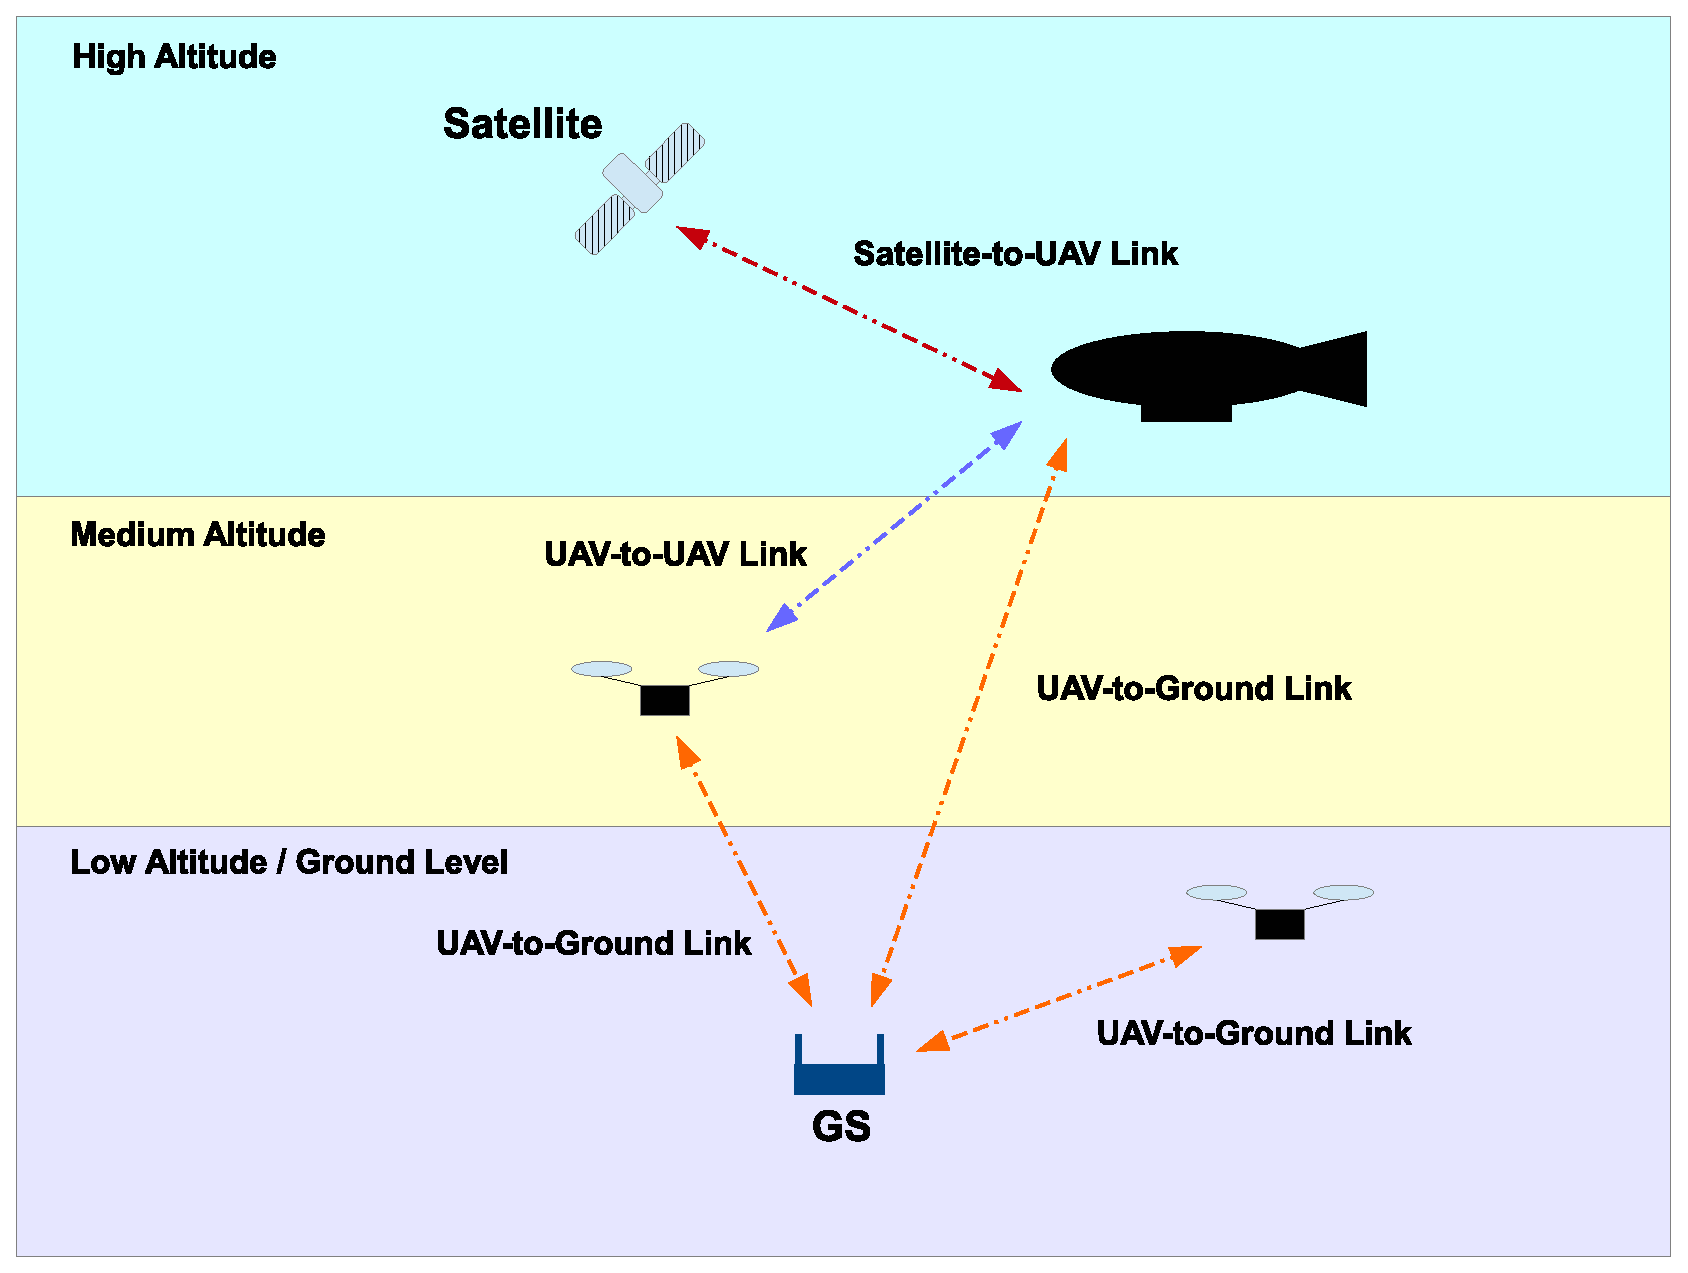
\includegraphics [width=0.49\columnwidth]{chap2_fig/multi_UAV_network_example.eps} 
\label{fig:lit_review_multi_UAV_network_example}}
\caption{An illustrated example of a MAV network and UAV network.}
\label{fig:lit_review_multi__UAV_MAV_network_example}
\end{figure*}

Nonetheless, when operated in a network, UAV and MAV networks \textcolor{black}{are similar} (Fig. \ref{fig:lit_review_multi__UAV_MAV_network_example}). For instance, the multi-MAV network depicted in Fig. \ref{fig:lit_review_multi_MAV_network_example} shows an example of the airport link, Air-to-Ground, Air-to-Air, and Satellite-to-Air communications from ground level to a high altitude. Specifically, communications between the airport GS and the MAVs, i.e., aircraft, can occur at the ground level when the aircraft is stationary or moving on the tarmac \cite{bartoli2013aeromacs}. At low to high altitude, MAVs can also communicate with the airport GS when en-route or arriving at the destination airport. MAVs can also communicate with other MAVs or satellite for navigational purposes. 

Similarly, the multi-UAV network in Fig. \ref{fig:lit_review_multi_UAV_network_example} shows an example of UAV-to-Ground, UAV-to-UAV, and Satellite-to-UAV communications from ground level to a high altitude. In particular, communications between the GS or satellite and the UAVs can take place due to CNPC or non-CNPC transmissions. Depending on the type of application, UAVs can also transmit CNPC or non-CNPC data to other UAVs.

Given the similarities between UAV and MAV networks, the focus of this chapter will be on UAV communications. In particular, with considerable flight time, payload weight, and range of MAVs, MAV networks can be viewed as a specific type of UAV network. Therefore, the work in this chapter is also applicable for MAV communications.



In the literature, UAVs have seen increased interest for various purposes, including the surveying of terrain \cite{andre2014application}, telecommunications relaying \cite{azari2018ultra}, and vehicular communications \cite{xiao2018uav,xiao2018user}. In particular, the deployment of multi-UAV networks, i.e., swarms of UAVs, has received substantial interest from both industry and academia as a means towards addressing the limited payload and flight time of individual UAVs \cite{andre2014application} and the lack of link redundancy in single-UAV networks \cite{wang2017taking}. Already, the deployment of multiple UAVs in the same network as flying base stations has been studied as a means to provide cellular service for ground users \cite{mozaffari2017wireless}.

% Elaborate on the purpose of this survey and contrast it with other UAV-related surveys.
However, in light of the spectrum scarcity challenge and technical limitations associated with UAV communications, accurate and realistic modeling of an HBD-UCS is required before any potential \textcolor{black}{solution} can be explored. In the literature, extensive research has been carried out for various aspects of UAV communications. In \cite{gupta2015survey}, several aspects of UAV communications were surveyed, including the characterization of UAV network types, routing protocol requirements in multi-UAV networks, handoff schemes in multi-UAV networks, and energy efficiency algorimths in UAV communications at the physical, data link, and network layers. In \cite{motlagh2016low}, a survey discussing the delivery of Internet of Things (IoT) services with UAVs was noted. Specifically, the authors discussed several use cases and architectures for UAV-based IoT service delivery, UAV-related regulatory requirements, along with the associated technical challenges. In a survey paper presented by Hayat et al. \cite{hayat2016survey}, the characteristics, applications, and requirements of multi-UAV networks were discussed from a communications perspective. Several candidate technologies that can potentially support UAV communications were also surveyed, including Bluetooth and WiFi, along with open research problems and challenges. Apart from these survey papers, similar works that surveyed UAV communications for integrated satellite-aerial-terrestrial networks \cite{liu2018space,cao2018airborne}, UAV-assisted wireless networks \cite{mozaffari2019tutorial}, UAV-based 5G and beyond networks \cite{li2018uav}, and UAV-assisted cellular networks \cite{fotouhi2019survey} have been noted. Recent survey papers on channel modeling in UAV communications have also been seen \cite{khuwaja2018survey,khawaja2019survey}.

\begin{figure} [tpb]
\centering
%\vspace{-2cm}
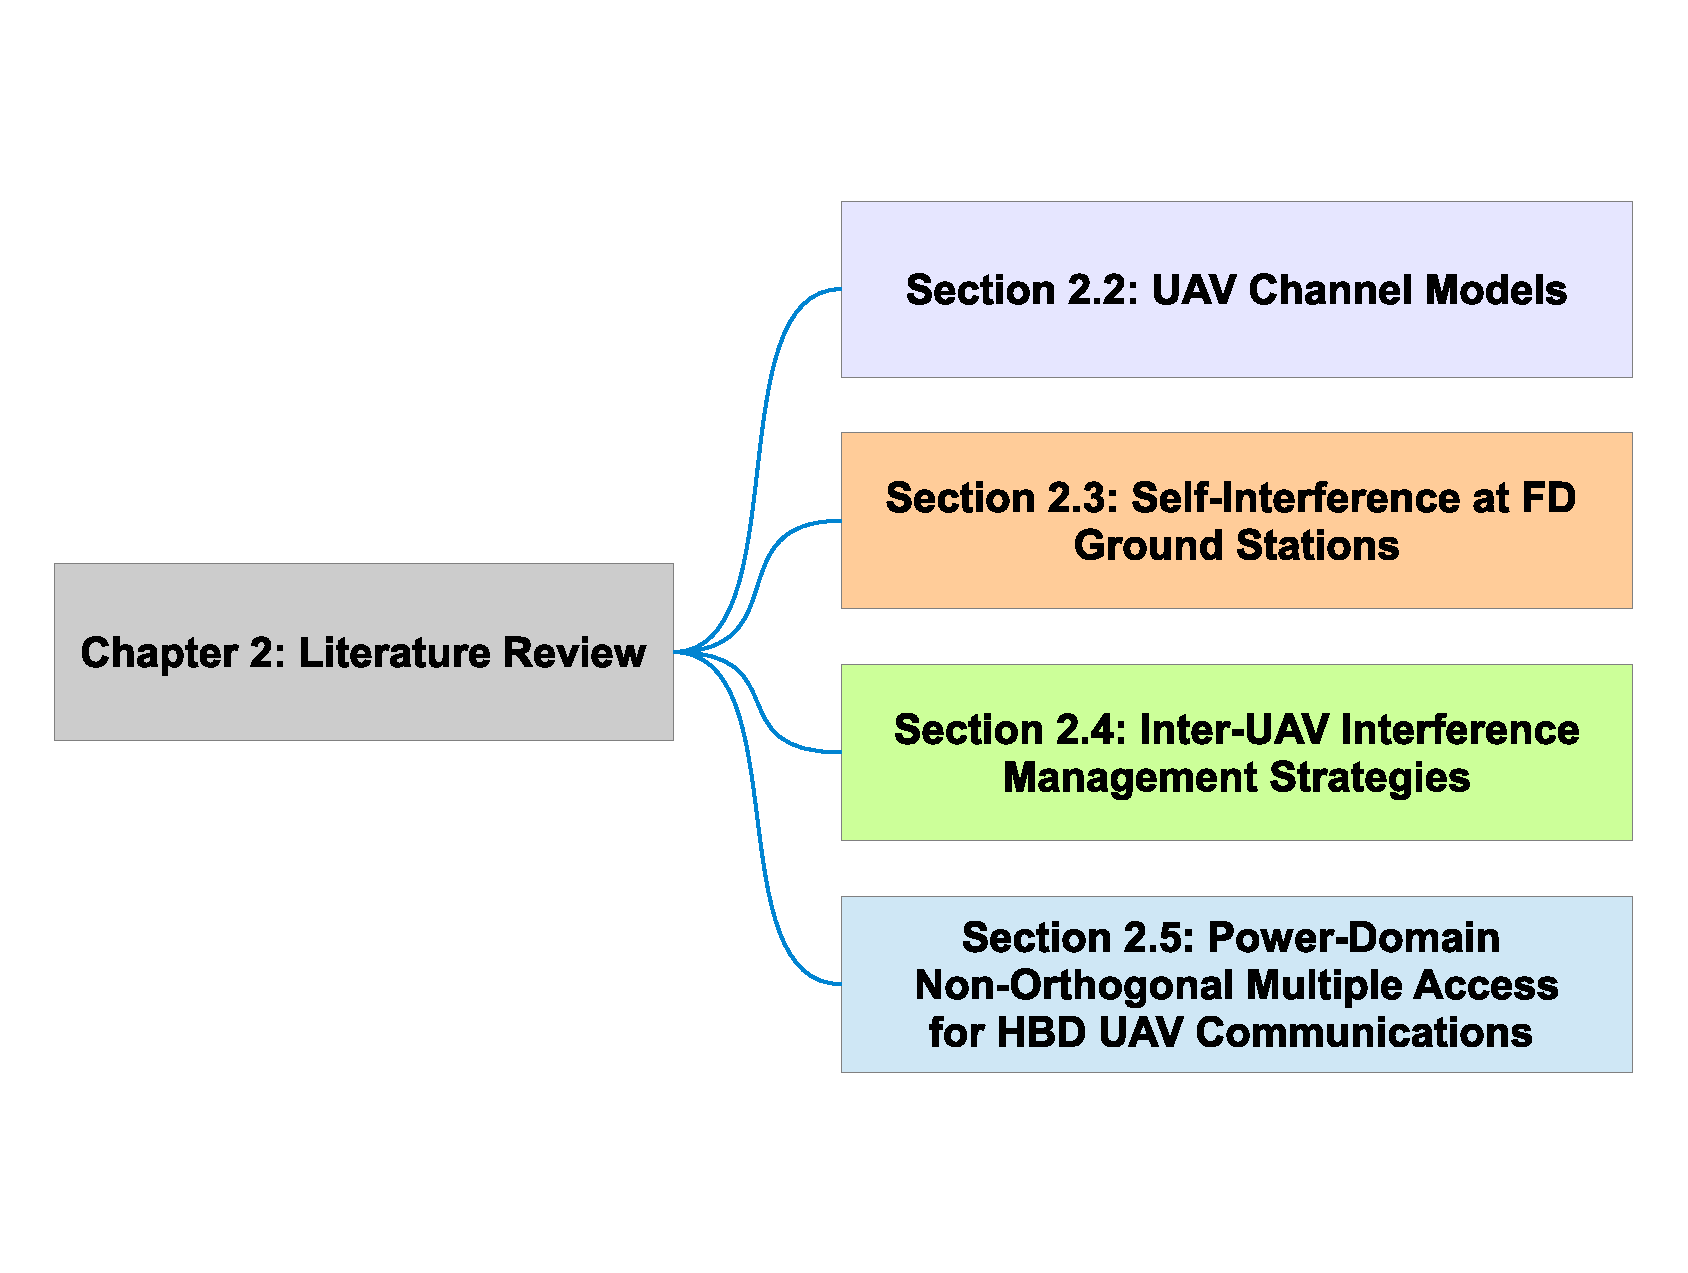
\includegraphics [width=0.8\columnwidth]{chap2_fig/taxonomy.eps} 
\vspace{-1cm}
\caption{The organization of the chapter.}
%\vspace{-0.5cm}
\label{fig:lit_review_taxonomy}
\end{figure}

% Detail our contributions and organization of this paper
While the above survey papers have discussed many different aspects of UAV communications, the issue of spectrum scarcity has mainly been ignored. In this spirit, this chapter discusses the associated challenges and opportunities in HBD UAV communications. The focus here is on FD-based networks to improve spectrum efficiency in UAV communications. 

The overall organization of this chapter is summarized in Fig. \ref{fig:lit_review_taxonomy}. In Section \ref{lit_review_sec_uav_chn}, the state-of-the-art related to UAV channel modeling is discussed, while Section \ref{lit_review_sec_si_fd_gs} presents SI mitigation architectures that can be used in HBD-UCSs. The various types of FD transceiver imperfections, along with accurate modeling of the impairments, are also discussed in Section \ref{lit_review_sec_si_fd_gs}. Interference management strategies that can be adopted at the HD UAVs are discussed in Section \ref{lit_review_sec_hd_uav_int}. Specifically, the state-of-the-art and the advantages and disadvantages for different interference management strategies, and its practical implementation and performance evaluation when used in an HBD-UCS, are surveyed in Section \ref{lit_review_sec_hd_uav_int}. In Section \ref{lit_review_sec_noma}, non-orthogonal multiple access (NOMA) methods are discussed to enable HBD-UCSs to support multi-UAV scenarios. Finally, the chapter is summarized in Section \ref{lit_review_sec_conclusion}.


% Present organization of the paper
%The remainder of this paper is organized as follows. The proposed system model is introduced in Section II, with outage probability and finite SNR diversity gain derivations for the joint detector presented in Section III and Section IV, respectively. The results of the numerical analysis are presented in Section V before the conclusion of the paper in Section VI.

%%%%%%%%%%%%%%%%%%%%%%%%%%%%%%%%%%%%%%%%%%%%%%%%%%%%%%%%%%%%%%%%%%%%%%%%%%%%%%%%%%%%%%%%%%%%%%%%%%%%%%%%%%%%%%%%%%%%%%%%%%%%%%%%%%%%%%%%%
% Section 2 : System Model
\section{UAV Channel Models} \label{lit_review_sec_uav_chn}

\begin{figure} [tpb]
\centering
\vspace{-1.5cm}
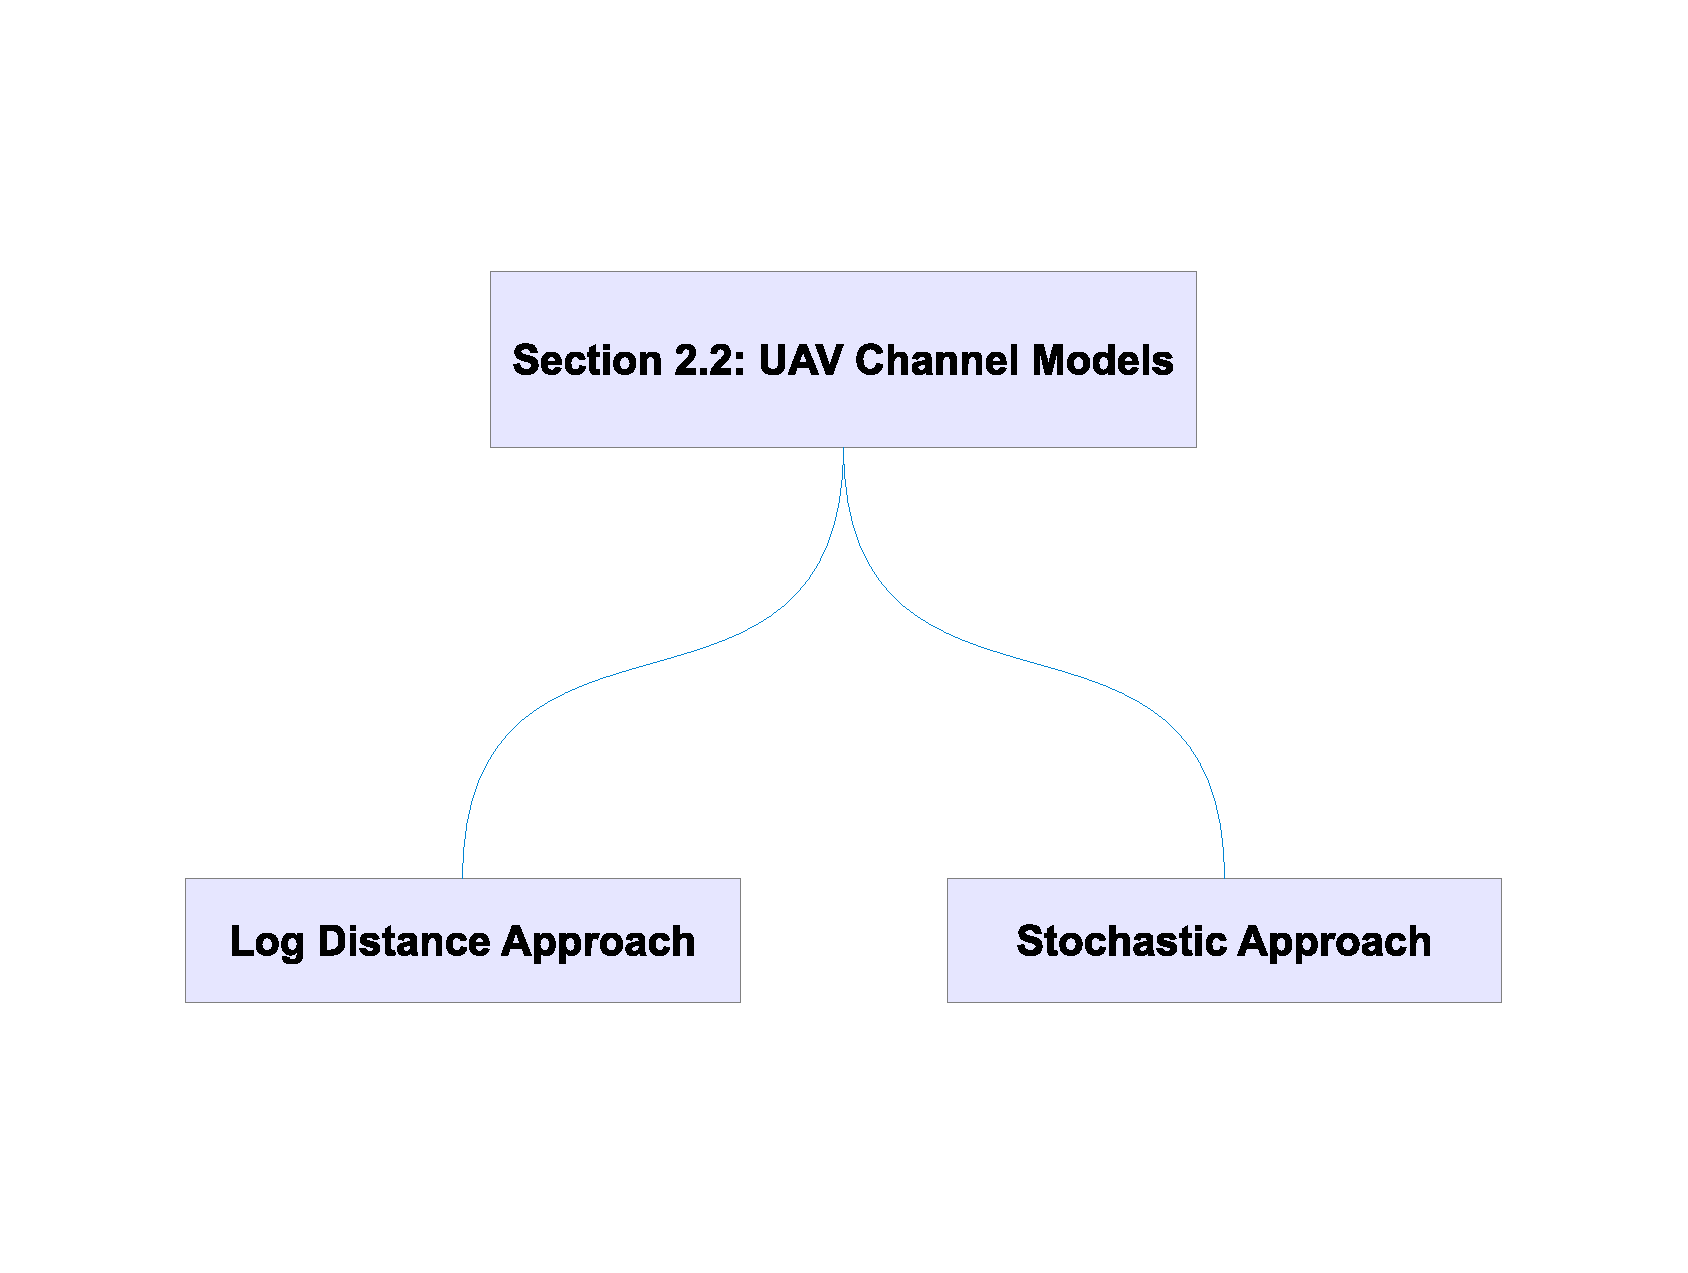
\includegraphics [width=0.8\columnwidth]{chap2_fig/sec_2_taxonomy.eps} 
\vspace{-2cm}
\caption{An overview of the topics in Section \ref{lit_review_sec_uav_chn}.}
%\vspace{-0.5cm}
\label{fig:lit_review_sec_2_taxonomy}
\end{figure}

With UAVs operating in various types of environments, e.g., urban environments, and flight domains, e.g., en route, CNPC and non-CNPC transmissions can occur over line-of-sight (LOS), and beyond-line-of-sight (BLOS) links \cite{kerczewski2012control}. As a result, the experienced QoS levels in UAV communications can vary. In this context, accurate UAV channel modeling is a prerequisite towards any meaningful evaluation of HBD UAV communications. With no single validated and widely accepted UAV channel model in the literature \cite{matolak2012air}, a review of UAV channel modeling is presented in this section (Fig. \ref{fig:lit_review_sec_2_taxonomy}) and summarized in Tables \ref{table:lit_review_stochastic_uav_channel_modeling} and \ref{table:lit_review_stochastic_uav_channel_modeling_adv_disadv}.

\subsection{Stochastic Approach} \label{lit_review_stochastic_approach}

\begin{summary} \emph{
\emph{The stochastic approach can be used to model UAV channels for specific scenarios/environments in the absence of available empirical data. However, the chosen statistical distribution of the UAV channel may not yield tractable expressions when computing performance metrics.}
}
\end{summary}

% Rayleigh Fading and Rician Fading in aeronautical communications
The stochastic approach to UAV channel modeling considers the effects of small scale fading in the channel model, such as Rayleigh or Rician fading. In \cite{haas2002aeronautical}, the aeronautical channel model was characterized for MAVs, i.e., aircraft, over various flight domains. In particular, Haas \cite{haas2002aeronautical} assumed that aeronautical communications took place over a Rayleigh fading channel if the LOS path is blocked, e.g., when the aircraft is parked at the terminal. On the other hand, a Rician fading channel is assumed if a clear LOS path exists between the aircraft and the GS, e.g., when the aircraft is en route. 

% Cite works modeling the UAV channel as a Rayleigh fading channel
% Introduce Rayleigh fading PDF
% Rayleigh fading assumption may not hold if due to operating altitude and terrain
For UAV communications, recent studies on modeling the UAV channel through the stochastic approach have also made similar assumptions. For instance, the link between the GS and the UAV is modeled as a Rayleigh fading channel in \cite{hayajneh2018performance,li2017optimal,lyu2017spectrum}. Let $|h|^2$ be the squared channel gain for a UAV channel $h$. Then, the PDF of $|h|^2$ for an UAV channel under Rayleigh fading is \cite[Table I]{rached2017unified}:
%%%%%%%%%%%%%%%%%%%%%%%%%%%%%%%%%%%%%%%%%%%%%%%%%%%%%%%%%%%%%%%%%%%%%%%%%%%%%%%%%
\begin{eqnarray} \label{lit_review_rayleigh_pdf}
f_{|h|^2}(x) = \frac{1}{\Omega}\exp\left(-\frac{x}{\Omega}\right),
\end{eqnarray}
%%%%%%%%%%%%%%%%%%%%%%%%%%%%%%%%%%%%%%%%%%%%%%%%%%%%%%%%%%%%%%%%%%%%%%%%%%%%%%%%%
where $\Omega$ represents the average received power. While Rayleigh fading can be used to model the worst-case effects of the propagation environment \cite{hayajneh2018performance} or UAV channels with blocked LOS links \cite{li2017optimal}, such assumptions may not necessarily hold due to the operating altitude and terrain. 

% Measurement campigns seen in Matolak's papers show that UAV channel can be modeled as a Rician fading channel. However, a piloted aircraft was used instead of an UAV. Therefore, empirical data may differ from actual propoation environment for small sized UAVs due to differences in velocity and altitude.
Measurement campaigns conducted for UAV communications over water \cite{matolak2017air_water}, hilly terrains \cite{sun2017air_hilly}, and urban environments \cite{matolak2017air_suburban} have shown that the link between the GS and the UAV, i.e., A/G link, can be modeled as a Rician fading channel. More importantly, the empirical approach was undertaken in \cite{matolak2017air_water,sun2017air_hilly,matolak2017air_suburban}, which has yielded meaningful insights into the Rician $K$ factor, path loss exponent, and delay spread that can be expected in the L-band and C-band. However, it must be pointed out that the measurement campaigns in \cite{matolak2017air_water,sun2017air_hilly,matolak2017air_suburban} were conducted with a piloted aircraft. Therefore, the range of essential parameters for a UAV channel, e.g., Rician $K$ factors, may differ from what was obtained from the empirical data due to differences in velocity and altitude between smaller sized UAVs and MAVs. 

% Rician fading is still a popular assumption. Cite works for Rician fading, do we cite VTC fall paper for rician fading?.
% Provide the PDF expression for Rician fading channel.
% Also cite work for UAV-to-UAV link being modeled as Rician fading
% Cite work for correlated Rician channel.
Nonetheless, the Rician fading assumption remains widely used in UAV channel modeling \cite{zeng2016wireless}. For a UAV channel under Rician fading, the PDF of $|h|^2$ is given as \cite[Table I]{rached2017unified}:
%%%%%%%%%%%%%%%%%%%%%%%%%%%%%%%%%%%%%%%%%%%%%%%%%%%%%%%%%%%%%%%%%%%%%%%%%%%%%%%%%
\begin{eqnarray} \label{lit_review_rician_pdf}
f_{|h|^2}(x) = \frac{K+1}{\Omega} \exp\left(-K-\frac{K+ 1}{\Omega}x\right)I_{0}\left(2\sqrt{\frac{K(K+1)}{\Omega}x}\right),
\end{eqnarray}
%%%%%%%%%%%%%%%%%%%%%%%%%%%%%%%%%%%%%%%%%%%%%%%%%%%%%%%%%%%%%%%%%%%%%%%%%%%%%%%%%
where $K$, and $I_{0}\left(\cdot\right)$ are the Rician $K$ factor and the modified zero order Bessel function of the first kind \cite{gradshteyn2014table}, respectively.

The expression in (\ref{lit_review_rician_pdf}) has been used in \cite{sharma2017uav,ono2016wireless,azari2018ultra,tan2018ricianShad} to model the Rician fading UAV channel for A/G links. More interestingly, it was shown by Azari et al. \cite{azari2018ultra} that the Rician $K$ factor can be modeled as a function of the elevation angle $\theta$ (in radians), i.e., elevation-dependent, as:
%%%%%%%%%%%%%%%%%%%%%%%%%%%%%%%%%%%%%%%%%%%%%%%%%%%%%%%%%%%%%%%%%%%%%%%%%%%%%%%%%
\begin{eqnarray} \label{lit_review_rician_k}
K=A_1\cdot\exp\left({A_2\theta}\right),
\end{eqnarray}
%%%%%%%%%%%%%%%%%%%%%%%%%%%%%%%%%%%%%%%%%%%%%%%%%%%%%%%%%%%%%%%%%%%%%%%%%%%%%%%%%
where $A_1$ and $A_2$ are environment and frequency dependent constants, respectively. At higher altitudes, the likelihood of a direct LOS link (between a UAV and a GS) increases \cite{azari2018key} due to less obstruction from buildings and terrain. Therefore, the UAV channel model in \cite{azari2018ultra} is useful when taking the effect of LOS obstruction, i.e., non-line-of-sight (NLOS), into consideration. However, the main drawback is that the relationship between the Rician $K$ factor and the elevation angle becomes environment-dependent \cite{azari2018ultra}. 

Apart from A/G links, the Rician fading assumption has also been used to model the UAV-to-UAV channel in recent literature, e.g., in \cite{goddemeier2015investigation,yuan2018capacity}. The authors in \cite{goddemeier2015investigation} considered the impact of altitude on the Rician fading UAV-to-UAV channel and showed that the Rician $K$ factor does not change significantly at high altitudes.
 
% conclude by saying that these PDF expressions will come in handy during the computation of relevant performance metrics, e.g., outage probability.
As seen from the earlier cited references in this subsection, the PDF expressions in (\ref{lit_review_rayleigh_pdf}) and (\ref{lit_review_rician_pdf}) are widely used in the literature for UAV channel modeling. Moreover, PDF expressions enable a better understanding of how the propagation environment impacts UAV communications and also crucial in the computation of relevant performance metrics, e.g., outage probability. One disadvantage of the stochastic approach is the intractability of expressions when computing certain performance metrics owing to the complexity of PDF expressions. However, the stochastic approach enables UAV channel models to be approximated through PDF expressions, e.g., using (\ref{lit_review_rayleigh_pdf}) and (\ref{lit_review_rician_pdf}), in the absence of readily available empirical data.

\subsection{Log Distance Approach} \label{lit_review_log_dist_approach}

\begin{summary}\emph{
\emph{The log distance approach accurately models UAV channels when empirical data are readily available. However, such an approach is heavily dependent on the assumed operating environment. Thus, UAV channel models obtained through the log distance approach are environment-specific.}
}
\end{summary}

% Introduce FSPL as one of the log distance approach, cite \cite{chandrasekharan2016designing,ITUR2013}
The log distance approach involves modeling the UAV channel by quantifying path loss due to the transmission distance and propagation environment. Such an approach has been used by the International Telecommunication Union (ITU-R) \cite{ITUR2013}, with free space path loss (FSPL) \cite{chandrasekharan2016designing} being a common assumption in recent research.

In \cite{feng2006path}, FSPL was assumed for the UAV channel, where the path loss is a function of the elevation angle and transmission distance in the A/G link. Feng et al. \cite{feng2006path} also modeled the effect of shadowing as a Normal distribution with zero mean and elevation-dependent standard deviation ($\sigma$) as:
%%%%%%%%%%%%%%%%%%%%%%%%%%%%%%%%%%%%%%%%%%%%%%%%%%%%%%%%%%%%%%%%%%%%%%%%%%%%%%%%%
\begin{eqnarray}
\sigma=B_1({90-\theta})^{B_2},
\end{eqnarray}
%%%%%%%%%%%%%%%%%%%%%%%%%%%%%%%%%%%%%%%%%%%%%%%%%%%%%%%%%%%%%%%%%%%%%%%%%%%%%%%%%
where $B_1$ and $B_2$ are obtained through curve fitting for the environment of interest. In \cite{al2014optimal}, FSPL was also assumed for the A/G link, with shadowing and scattering modeled as a Gaussian random variable (RV). Unfortunately, the effects of small scale fading are not considered in \cite{feng2006path} and \cite{al2014optimal}. Thus, the analysis in \cite{feng2006path,al2014optimal} cannot be readily applied for low altitude UAV channel models since small scale fading is likely to occur. In \cite{mozaffari2017wireless}, the authors assumed FSPL for both LOS and NLOS links in the UAV channel model. The amount of FSPL is taken as a function of the ground receiver's location. Additionally, Mozaffari et al. \cite{mozaffari2017wireless} assumed the probability of the UAV channel encountering LOS and NLOS links to be elevation-dependent in the A/G link using the following relationship:
%%%%%%%%%%%%%%%%%%%%%%%%%%%%%%%%%%%%%%%%%%%%%%%%%%%%%%%%%%%%%%%%%%%%%%%%%%%%%%%%%
\begin{eqnarray}
Pr(LOS) & = & b_1 \left(\frac{180}{\pi}\theta - 15\right)^{b_2} \\
Pr(NLOS) & = & 1- Pr(LOS),
\end{eqnarray}
%%%%%%%%%%%%%%%%%%%%%%%%%%%%%%%%%%%%%%%%%%%%%%%%%%%%%%%%%%%%%%%%%%%%%%%%%%%%%%%%% 
where $b_1$ and $b_2$ are environment-dependent constants. 

%\begin{sidewaystable}
\begin{table*}[]
\centering
\caption{Summary of UAV Channel Modeling Considerations}
\label{table:lit_review_stochastic_uav_channel_modeling}
\scalebox{0.7}{
\begin{tabular}{llllll}
\hline
Reference														& Approach			& Small Scale Fading Model 	& Shadowing Model		& UAV Velocity Model	& UAV Spatial Model \\ \hline \hline
 \cite{mozaffari2017wireless}				& Log Distance	& -													&	-									& -										& Gaussian 	\\
 \cite{azari2018ultra}							& Stochastic		& Rician										& -									& -										& PPP 			\\
 \cite{hayajneh2018performance,li2017optimal}	&	Stochastic		&	Rayleigh 				& -									& -										& PPP 			\\
 \cite{lyu2017spectrum}							& Stochastic		& Rayleigh									& -									& -										& - 				\\ 
 \cite{sharma2017uav,ono2016wireless}	&	Stochastic	& Rician										& -									& Constant 						& - 				\\
 \cite{tan2018ricianShad}						& Stochastic		& Rician Shadowed						& Rician Shadowed		& - 									& - 				\\
 \cite{goddemeier2015investigation} & Stochastic		& Rician										& -									& -										& - 				\\
 \cite{yuan2018capacity}						& Stochastic		& Rician										& -									& Constant 						& ST Mobility Model \cite{wan2013smooth}	\\
 \cite{feng2006path,al2014optimal}	& Log Distance	& -													& Gaussian					& - 									& - 				\\
 \cite{al2017modeling,amorim2017radio}	& Log Distance	& -											& Gaussian					& -										& - 				\\
 \cite{pokkunuru2017capacity}				& Log Distance	& Rician, Rayleigh					& Gaussian					& Gaussian						& Uniform 	\\
 \cite{sallouha2017aerial}					& Log Distance	& -													& Log Normal				& -										& - 				\\ \hline
\end{tabular}}
\end{table*}

\begin{table*}[]
\centering
\caption{Summary of Advantages and Disadvantages of the UAV Channel Modeling Approaches}
\label{table:lit_review_stochastic_uav_channel_modeling_adv_disadv}
\scalebox{0.7}{
\begin{tabular}{lll}
\hline
Approach			& Advantage  																													& Disadvantage  \\ \hline \hline
Stochastic		& Uses well-known statistical distributions to model the UAV channel. & Analysis may be intractable. \\
Log Distance	& Accurately models UAV channels with empirical data. 								& Environment-specific. \\ \hline
\end{tabular}}
\end{table*}

It must be pointed out that depending on the operating environment, the FSPL assumption might not always hold due to larger path loss exponents. To this end, recent works have adopted a general log distance approach to consider arbitrary path loss exponent values as follows:
%%%%%%%%%%%%%%%%%%%%%%%%%%%%%%%%%%%%%%%%%%%%%%%%%%%%%%%%%%%%%%%%%%%%%%%%%%%%%%%%%
\begin{eqnarray} \label{lit_review_path_loss}
L(d)=n\cdot10\log\left({d}/{d_0}\right) + C + X,
\end{eqnarray}
%%%%%%%%%%%%%%%%%%%%%%%%%%%%%%%%%%%%%%%%%%%%%%%%%%%%%%%%%%%%%%%%%%%%%%%%%%%%%%%%%
where $L(d)$ is the path loss in dB from distance $d$ in meters, $d_0 = 1$ is the reference distance, $n$ is the path loss exponent, $C$ is a constant dependent on antenna gain and path loss from distance $d_0$, and $X$ is a RV representing excess path loss. 

In \cite{al2017modeling} and \cite{amorim2017radio}, path loss is modeled using (\ref{lit_review_path_loss}) in the UAV channel model. Shadowing is also modeled in \cite{al2017modeling} by letting $X$ be a zero mean Gaussian RV, with elevation-dependent standard deviation taken as:
%%%%%%%%%%%%%%%%%%%%%%%%%%%%%%%%%%%%%%%%%%%%%%%%%%%%%%%%%%%%%%%%%%%%%%%%%%%%%%%%%
\begin{eqnarray}
\sigma=B_1\theta + B_2.
\end{eqnarray}
%%%%%%%%%%%%%%%%%%%%%%%%%%%%%%%%%%%%%%%%%%%%%%%%%%%%%%%%%%%%%%%%%%%%%%%%%%%%%%%%%
In \cite{pokkunuru2017capacity}, the authors modeled the UAV channel by combining the effect of path loss, gaseous absorption, shadowing, Doppler spread, and small scale fading. However, only arbitrary path loss exponents were considered for the NLOS link in the UAV channel model, with FSPL assumed for the LOS link. In \cite{sallouha2017aerial}, the log distance approach was assumed for an A/G UAV channel in a suburban environment. Sallouha et al. \cite{sallouha2017aerial} also considered the impact of the elevation angle ($\theta$) on the probability of LOS occurrence $\big(Pr(LOS)\big)$ and the path loss exponent $(n)$ through the following relationship:
%%%%%%%%%%%%%%%%%%%%%%%%%%%%%%%%%%%%%%%%%%%%%%%%%%%%%%%%%%%%%%%%%%%%%%%%%%%%%%%%%
\begin{eqnarray}
Pr(LOS) & \approx & \frac{1}{1+b_1\exp\left(-b_2\theta\right)}, \\
n & = & (2-B_3)Pr(LOS) + B_3,
\end{eqnarray}
%%%%%%%%%%%%%%%%%%%%%%%%%%%%%%%%%%%%%%%%%%%%%%%%%%%%%%%%%%%%%%%%%%%%%%%%%%%%%%%%% 
where $B_3 \in [2.7,3.5]$.

One disadvantage of the approach undertaken in \cite{sallouha2017aerial}, along with earlier cited references in this subsection, is that the resultant UAV channel model is highly dependent on the operating environment. Thus, the insights gained from log distance-based UAV channel models in suburban environments may not necessarily apply for UAV channel models in other environments, e.g., over hilly terrains. Nevertheless, the log distance approach is still useful in modeling UAV channels for specific environments where empirical data can be readily obtained.

%%%%%%%%%%%%%%%%%%%%%%%%%%%%%%%%%%%%%%%%%%%%%%%%%%%%%%%%%%%%%%%%%%%%%%%%%%%%%%%%%%%%%%%%%%%%%%%%%%%%%%%%%%%%%%%%%%%%%%%%%%%%%%%%%%%%%%%%%
% Section 3 : Outage Probability
\section{Self-Interference at FD Ground Stations} \label{lit_review_sec_si_fd_gs}

\begin{figure} [tpb]
\centering
%\vspace{-1cm}
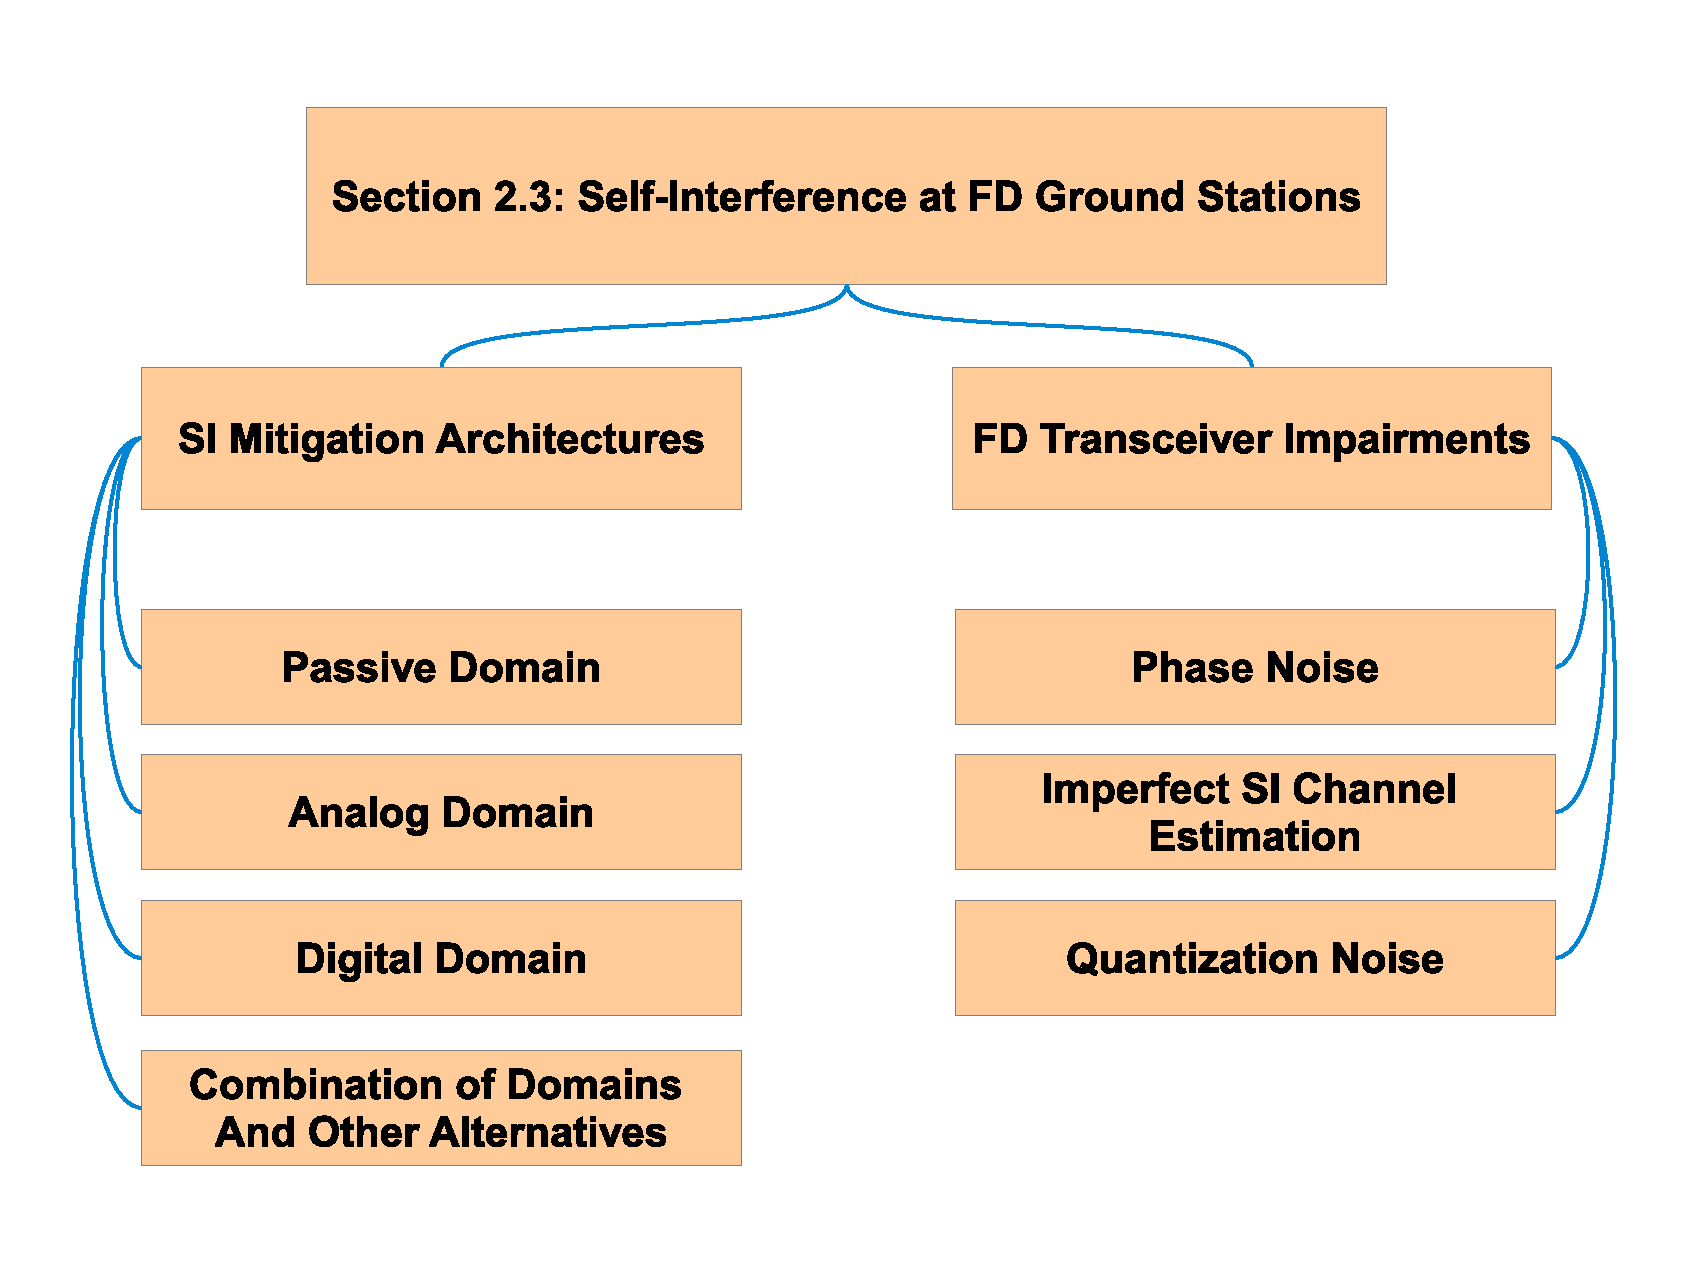
\includegraphics [width=0.8\columnwidth]{chap2_fig/sec_3_taxonomy.eps} 
\vspace{-0.5cm}
\caption{An overview of the topics in Section \ref{lit_review_sec_si_fd_gs}.}
%\vspace{-0.5cm}
\label{fig:lit_review_sec_3_taxonomy}
\end{figure}

As GSs operate in FD mode in HBD UAV communications, SI at GSs must be modeled accurately to enable a meaningful performance analysis. To this end, a review of SI mitigation architectures and the impairments associated with FD transceivers are provided in this section (Fig. \ref{fig:lit_review_sec_3_taxonomy}).

\subsection{SI Mitigation Architectures}
\begin{summary} \emph{
\emph{SI mitigation architectures operate in the passive, analog, or digital domain. Architectures that involve combinations of different domains are also possible. However, SI cannot be completely removed due to FD transceiver impairments.}
}
\end{summary}

\begin{figure} [h]
\centering
%\vspace{-1.5cm}
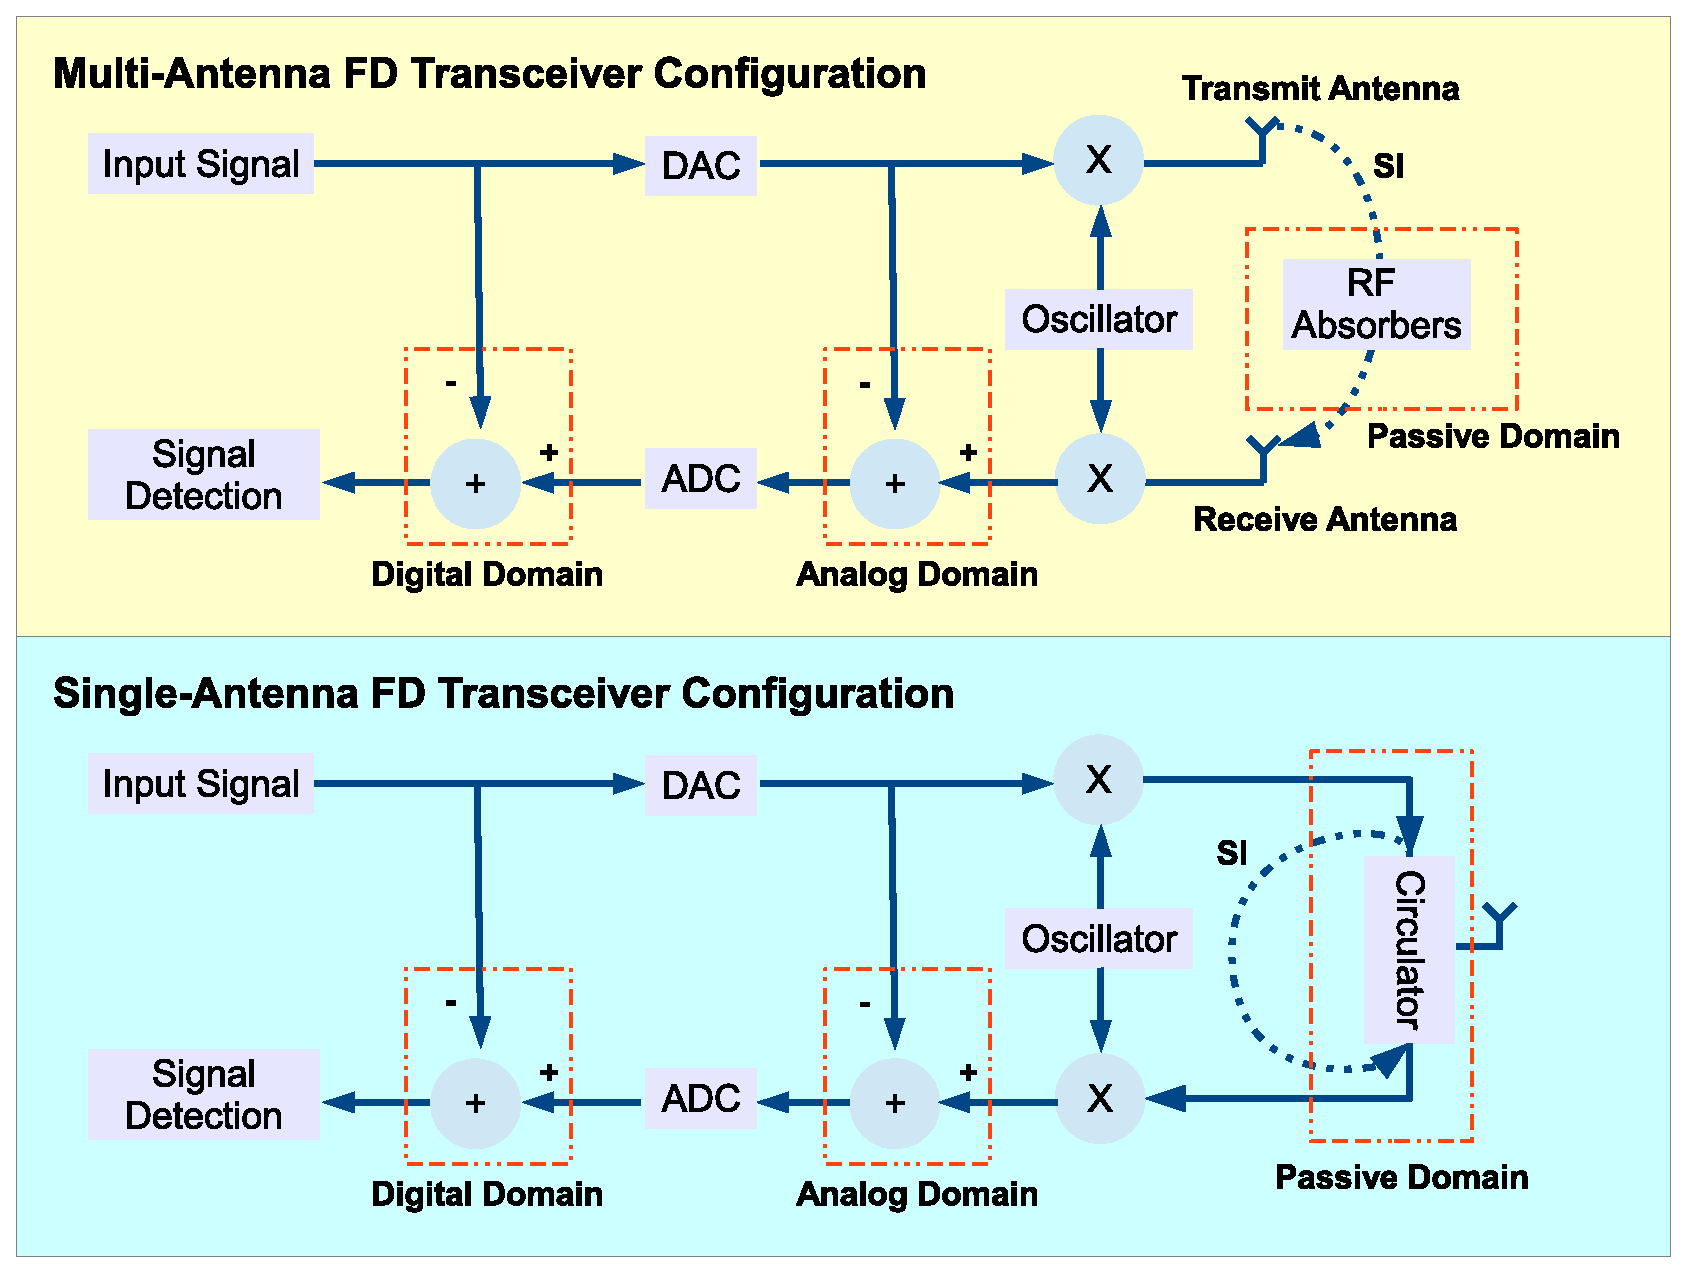
\includegraphics [width=0.6\columnwidth]{chap2_fig/SI_mitigation_example.eps} 
%\vspace{-1.5cm}
\caption{An example of SI mitigation in multi-antenna and single-antenna FD transceivers. For both configurations, SI mitigation through combinations of passive, analog, and digital domain techniques are possible.}
%\vspace{-0.5cm}
\label{fig:lit_review_SI_mitigation_example}
\end{figure}

Mitigating SI in FD transceivers is a topic that has been widely investigated in the literature. In particular, a wide body of works has investigated SI mitigation architectures that operate in different signal domains. Alternative approaches, such as beamforming, have also been proposed. The principles and tradeoffs associated with the various architectures are presented below. A summary of studies on SI mitigation architectures is also provided in Table \ref{table:lit_review_si_mitigation_arch2}.

\subsubsection{Passive Domain}
SI mitigation architectures operating in the passive domain suppresses SI through the inducement of pathloss. For multi-antenna FD transceivers, pathloss can be induced through antenna separation and placement of radio frequency (RF) absorbers \cite{everett2014passive}. The use of balanced/unbalanced (Balun) transformers has also been discussed \cite{jain2011practical}. On the other hand, circulators and duplexers are used to isolate the transmit and receive chains in single-antenna FD transceivers \cite{korpi2016full}. Specifically, a circulator restricts transmit chain signals from interfering with receive chain signals, e.g., Fig. \ref{fig:lit_review_SI_mitigation_example}, while a duplexer undergoes tuning to match the impedance of the antenna. In \cite{amjad2018low}, an antenna patch for a single-antenna FD transceiver configuration was designed to mitigate SI in the passive domain without the need for circulators and duplexers.

Although it has been shown that SI can be mitigated in the passive domain, there are still drawbacks associated with passive domain techniques. Multi-antenna FD transceivers suffer from a reduction in overall spectrum efficiency since antennas are dedicated to either transmit or receive signals \cite{amjad2018low}. For single-antenna FD transceivers, circulators may cause the overall size of the transceiver to be substantial due to the wavelength of the signal's frequency \cite{korpi2016full}. In contrast, duplexers can be smaller in size. However, frequent tuning is still required, thus reducing overall spectrum efficiency. 

In the context of HBD UAV communications, passive domain techniques may be feasible in specific operating environments, e.g., FD-enabled GSs in urban environments. However, such techniques may not be cost-effective and suffer from limited SI mitigation capabilities \cite{amjad2018low}. Nonetheless, it must be noted that the size and power requirements for FD-enabled GSs may not be as stringent. Thus, the effectiveness of passive domain SI mitigation architecture can be further investigated for FD-enabled GSs in HBD UAV communications.

\subsubsection{Analog Domain}
For SI mitigation architectures operating in the analog domain, SI is mitigated before the receive chain signal enters the transceiver's analog-to-digital converter (ADC). In particular, the SI cancellation signal is first generated by taking a copy of the transmit chain signal at the output of the transceiver's digital-to-analog converter (DAC), e.g., Fig. \ref{fig:lit_review_SI_mitigation_example}. Such an approach enables the SI cancellation signal to retain the same transceiver impairments of the SI signal, such as oscillator phase noise. \textcolor{black}{Thereafter, the SI cancellation signal is added to the incoming receive chain signal to remove SI}. Examples of works that have investigated SI mitigation in the analog domain include \cite{sahai2013impact,ahmed2013rate}, and \cite{syrjala2016analysis}. 

Although analog domain SI mitigation architectures have been widely studied, overcoming the associated limitations remains a challenge. The cost, size, and power consumption of the FD transceivers may increase when considering SI mitigation in the analog domain \cite{bernhardt2018self}. Furthermore, SI cancellation in the analog domain is limited by transceiver impairments, such as imperfect SI channel estimation and  phase noise \cite{sahai2013impact}.

Despite the limitations, implementing analog domain SI mitigation, in the context of HBD UAV communications, is an interesting research problem of practical significance. For instance, analog domain SI mitigation architectures at FD-enabled GSs can be investigated to understand potential cost and power requirements. Understanding such requirements will be beneficial towards an evaluation of development and operational feasibility for HBD UAV communications.

\begin{table*}[]
\centering
\caption{Summary of Studies on SI Mitigation Architectures}
\label{table:lit_review_si_mitigation_arch2}
\scalebox{0.7}{
\begin{tabular}{lllll}
\hline
Reference										& Domain 																									& SI Suppression						& RF Chain Configuration	& SI Channel Model		\\ \hline \hline
\cite{ernest2019outage}			& Analog, Digital																					& 163 dB to 175 dB					& Separate								& Rician Fading 			\\
\cite{tan2018joint}					& Analog, Digital																					& 163 dB to 175 dB					& Separate								& Rician Fading 			\\
\cite{ernest2019power}			& Analog, Digital																					& 163 dB										& Separate								& Rician Fading 			\\
\cite{ernest2019hybrid}			& Analog, Digital																					& 174 dB to 181 dB					& Separate								& Rician Fading 			\\
\cite{sahai2013impact}			& Analog, Digital																					&	35 dB to 60 dB (Analog),	& WARP \cite{warp2019}, 	& Rayleigh Fading 		\\ 
														& 																												&	0 dB to 32 dB (Digital)		& Vector Signal 					& 										\\
														&																													&														& Generator \cite{esg2019}&											\\
\cite{everett2014passive}		& Passive (Antenna Separation,														& 24.5 dB to 73.8 dB				&	Separate								&	Rician Fading, 			\\
														&	RF Absorbers)																						&														&													& Rayleigh Fading 		\\
\cite{jain2011practical}		& Passive (Balun)																					& 40 dB to 52 dB						&	Separate								&	Rayleigh Fading			\\
\cite{korpi2016full}				&	Passive (Circulators, 																	&	20 dB to 22 dB 						&	Single									& Non-linear					\\
														& Duplexers)																							&														&													&											\\
\cite{amjad2018low} 				& Passive (Single-Patch Antenna), 												&	56 dB to 60 dB (Passive)	&	Single									& Frequency-selective \\
														&	Digital																									&														&													&	Rayleigh Fading			\\ 
														& 																												&	14 dB to 35 dB (Digital)	&													& 										\\
														& 																												&	84 dB to 88 dB (Total)		&													& 										\\ 
\cite{ahmed2013rate}				& Analog, Digital																					& 20 dB to 60 dB (Passive)	& Separate								& Rician Fading 			\\ 
\cite{syrjala2016analysis}	& Analog, Digital																					&	60 dB to 110 dB (Total)		& Separate								& Multipath 					\\
\cite{bernhardt2018self} 		& Others (Advanced Sampling)															& 35 dB											& Separate								& Rician Fading 			\\
\cite{korpi2014full}				& Digital																									& 35 dB											& Separate								& Static Multipath 		\\ 
\cite{ahmed2015all}					& Digital																									& 25 dB to 60 dB (Passive)	& Separate								& Rician Fading 			\\ 
\cite{li2018self}						& Digital																									&	20 dB to 60 dB						& Separate								& Rayleigh Fading \\ 
\cite{shende2018half}				& Analog, Digital																					& -													& Separate								& Rayleigh Fading 		\\  
\cite{hwang2017multi}				& Others (Beamforming)																		& - 												& Separate								& Multipath 					\\ 
\cite{chalise2017beamforming}	& Others (Beamforming)																	& -													& Separate								& Rayleigh Fading 		\\ 
\cite{mohammadi2018beamforming}	&	Others (Beamforming)																& -													& Separate								& Rayleigh Fading \\ \hline
\end{tabular}}
\end{table*}

\subsubsection{Digital Domain}
For digital domain SI mitigation architectures, SI is mitigated after the receive chain signal exits the transceiver's ADC. Specifically, the SI cancellation signal is generated using a copy of the transmit chain signal at the input of the transceiver's ADC (Fig. \ref{fig:lit_review_SI_mitigation_example}). Similar to analog domain SI mitigation, the SI cancellation signal in the digital domain also retains the same transceiver impairments as the SI signal. SI is then mitigated by adding the SI cancellation signal to the receive chain signal at the output of the transceiver's ADC. Studies that have adopted such an approach include \cite{amjad2018low,sahai2013impact,ahmed2013rate,syrjala2016analysis,korpi2014full,ahmed2015all,li2018self}.

With extensive studies on digital domain SI mitigation architectures noted in the literature, some techniques have achieved substantial amounts of SI cancellation \cite{bernhardt2018self}. Nonetheless, there are several limitations associated with SI cancellation in the digital domain. Similar to analog domain techniques, digital domain SI cancellation is also limited by phase noise and imperfect SI channel estimation. In particular, the latter affects the quality of the SI cancellation signal since an imperfect SI channel estimate leads to inaccurate modeling of the actual SI signal \cite{amjad2018low}. In addition to phase noise and imperfect SI channel estimation, the dynamic range of the ADC is another key constraint in digital domain techniques. With a limited dynamic range, the input of the ADC is mostly dominated by the SI instead of the desired signal when the SI power is high \cite{ahmed2013rate,korpi2014full}. As a result, the desired signal becomes overwhelmed by quantization noise \cite{bernhardt2018self}. Other associated limitations include transceiver nonlinearities \cite{ahmed2015all} and in-phase/quadrature (IQ) imbalance \cite{li2018self}.

Addressing the limitations of digital domain SI mitigation remains an interesting research problem. These issues must be adequately investigated before the practical implementation of FD-enabled GSs in HBD UAV communications.

\subsubsection{Combination of Domains and Other Alternative Approaches}
%%%%%%%%%%%%%%%%%%%%%%%%%%%%%%%%%%%%%%%%%%%%%%%%%%%%%%%%%%%%%%%%%%%%%%%%%%%%%%%%%
% Apart from focusing on SI mitigation techniques that operate in a specific domain, SI mitigation that involves the combination of techniques from difference domains have been seen in the literature. 
% For instance, Amjad et al. \cite{amjad2018low} combined passive suppression, through a proposed antenna design, with digital SI mitigation to achieve 88 dB of SI suppression.
% Separately, other studies, e.g., \cite{sahai2013impact,ahmed2013rate,shende2018half,ernest2019outage,tan2018joint}, have assumed a combination of analog and digital SI cancellation operating in cascade. Specifically, the SI signal undergoes SI mitigation in the analog domain first, before SI cancellation in the digital domain. To account for FD transceiver impairments, residual SI is considered in the signal models of \cite{sahai2013impact,ahmed2013rate,shende2018half,ernest2019outage,tan2018joint}. The strength of the residual SI depends on a variety of factors, including the variance of the phase noise \cite{sahai2013impact,ahmed2013rate,ernest2019outage,tan2018joint}, variance of the SI channel estimation error \cite{sahai2013impact,ahmed2013rate,ernest2019outage,tan2018joint,zlatanov2017capacity}, quantization noise \cite{ahmed2013rate}, and transmit power \cite{shende2018half}.
% Other than techniques that focuses on SI cancellation, other innovative solutions have also been pursued. Beamforming, for example, has been studied in \cite{hwang2017multi,chalise2017beamforming,mohammadi2018beamforming} to suppress SI while an advanced sampling technique that avoids sampling the SI signal was proposed in \cite{bernhardt2018self}. However, it still remains to be seen if these techniques, e.g., beamforming or advanced sampling, can be realistically implemented owing to the associated computational complexity and hardware cost. 
%%%%%%%%%%%%%%%%%%%%%%%%%%%%%%%%%%%%%%%%%%%%%%%%%%%%%%%%%%%%%%%%%%%%%%%%%%%%%%%%%
Apart from focusing on SI mitigation techniques that operate in a specific domain, SI mitigation that involves the combination of techniques from different domains have been seen in the literature. For instance, Amjad et al. \cite{amjad2018low} combined passive suppression, through a proposed antenna design, with digital SI mitigation to achieve 88 dB of SI suppression.

Separately, other studies, e.g., \cite{ernest2019outage,tan2018joint,ernest2019power,sahai2013impact,ahmed2013rate,shende2018half}, have assumed a combination of analog and digital SI cancellation operating in cascade. Specifically, the SI signal undergoes SI mitigation in the analog domain first, before SI cancellation in the digital domain. To account for FD transceiver impairments, residual SI is considered in the signal models of \cite{ernest2019outage,tan2018joint,ernest2019power,sahai2013impact,ahmed2013rate,li2018self,shende2018half}. The strength of the residual SI depends on a variety of factors, including the variance of the phase noise \cite{ernest2019outage,tan2018joint,ernest2019power,sahai2013impact,ahmed2013rate,li2018self}, variance of the SI channel estimation error \cite{ernest2019outage,tan2018joint,ernest2019power,sahai2013impact,ahmed2013rate,zlatanov2017capacity}, quantization noise \cite{ahmed2013rate}, and transmit power \cite{shende2018half}.

Other than techniques that focus on SI cancellation, innovative solutions have also been pursued. Beamforming, for example, has been studied in \cite{hwang2017multi,chalise2017beamforming,mohammadi2018beamforming} to suppress SI while an advanced sampling technique that avoids sampling the SI signal was proposed in \cite{bernhardt2018self}. However, it remains to be seen if these techniques, e.g., beamforming or advanced sampling, can be realistically implemented owing to the associated computational complexity and hardware cost.

\subsection{Modeling FD Transceiver Impairments in HBD UAV Communications}
\begin{summary} \emph{
\emph{Accurate modeling of FD transceiver impairments, e.g., phase noise, imperfect SI channel estimation errors, and quantization noise can be used to gauge the strength of residual SI in FD transceivers.  
}}
\end{summary}
As impairments are present in FD transceivers, realistic modeling of the imperfections is required to enable a sound analysis of HBD UAV communications. To this end, some of the impairments that are commonly found in the literature are discussed below. 

\subsubsection{Phase Noise}
In FD transceivers, phase noise stems from the jitter present in the oscillator \cite{sahai2013impact}. Depending on the FD transceiver design, the strength of the phase noise can differ. FD transceivers with shared oscillators are impaired from the same phase noise source on both the transmit and receive RF chains \cite{li2018self,syrjala2014analysis}. In contrast, FD transceivers with separate oscillators for the transmit and receive RF chains are affected by two independent phase noise sources, thus leading to stronger phase noise \cite{li2018self}.

To account for phase noise in FD transceivers, one can adopt the models in \cite{ernest2019outage,tan2018joint,ernest2019power,sahai2013impact}. Specifically, let the phase noise term be $\gamma_{\phi} w_{\phi}$, where $w_{\phi}$ is a Gaussian RV with zero mean and unit variance, and $\gamma_{\phi}$ be a scaling factor. The scaling factor depends on the oscillator of interest. For instance, the transceivers (\textcolor{black}{transmit chain}) used in \cite[Appendix C]{sahai2013impact} have variance (denoted as $\sigma_{\phi}$ in \cite{sahai2013impact}) of $\gamma_{\phi}^2 = 0.717^{\circ} = 0.0125$ \textcolor{black}{radians} and $\gamma_{\phi}^2 = 0.066$. Furthermore, in \cite[Appendix C]{sahai2013impact}, $\sigma_{\phi}=2\pi f_c \Delta{t_{RMS}}$, where $f_c$ is carrier frequency and $\Delta{t_{RMS}}$ is the jitter in time. Thus, one can accurately model the strength of the phase noise based on the transceiver specifications such as the carrier frequency and jitter in time.

\subsubsection{Imperfect SI Channel Estimation}
In theory, SI can be eliminated if the full channel state information (CSI) of the SI channel is known. However, in practice, the SI channel is estimated using a training sequence \cite{ahmed2015all,sahai2013impact}. The inaccuracy of the SI channel estimation process invariably contributes to residual SI at the FD transceiver as the SI canceling signal is generated based on the estimated SI channel.
 
To model the imperfect SI channel estimation, one can adopt the model in \cite{zlatanov2017capacity}. In particular, let $\widetilde{h}_{si}$ be the error of the imperfect SI channel gain estimate, where $\widetilde{h}_{si}=h_{si}-\widehat{h}_{si}$, $h_{si}$ is the SI channel gain, and $\widehat{h}_{si}$ is the imperfect estimation of $h_{si}$. Furthermore, let $\widetilde{h}_{si}$ be modeled as a zero mean, circularly symmetric complex Gaussian RV with variance $\epsilon$ to quantify the SI channel estimation error \cite{zlatanov2017capacity}. The variance $\epsilon$ of $\widetilde{h}_{si}$ represents the accuracy of the measured CSI for the SI channel. It is worth noting that the same approach has been seen in \cite{wang2017sir} for the modeling of residual interference in wireless networks. By modeling $\widetilde{h}_{si}$ as a Gaussian RV, the worst case residual SI can be accounted in the FD transceiver \cite{zlatanov2017capacity}.

\subsubsection{Quantization Noise}
In FD transceivers, the quantization of the SI signal from the analog to the digital domain introduces noise to the overall SNR \cite{ahmed2015all,ahmed2013rate}. When the SI signal is strong, the dynamic range of the ADC becomes increasingly occupied by the SI signal, thus reducing the dynamic range available for the desired signal \cite{korpi2014full}. In turn, the performance of the FD transceiver is limited by quantization noise, since the ADC operates with a small number of bits, which masks the weak desired signal at the ADC output \cite{ahmed2013rate,bernhardt2018self}.

Quantization noise at an $m$-bit ADC can be modeled in terms of the low noise amplifier (LNA) as $\sigma_{ADC}^2 = \frac{1}{\alpha_{LNA} 12 \cdot 2^{2m-2}}$, where $\alpha_{LNA}$ denotes the LNA gain \cite{ahmed2015all,ahmed2013rate}. Based on the definition of $\sigma_{ADC}^2$, quantization noise can be effectively reduced by increasing the LNA gain ($\alpha_{LNA}$) or the number of bits ($m$) \cite{ahmed2015all}. However, having ADCs that can realistically operate with a large number of bits, e.g., $m>16$, is still an open research problem.

%%%%%%%%%%%%%%%%%%%%%%%%%%%%%%%%%%%%%%%%%%%%%%%%%%%%%%%%%%%%%%%%%%%%%%%%%%%%%%%%%%%%%%%%%%%%%%%%%%%%%%%%%%%%%%%%%%%%%%%%%%%%%%%%%%%%%%%%%
% Section: Interference at HD UAVs
\section{Inter-UAV Interference Management Strategies} \label{lit_review_sec_hd_uav_int}

\begin{figure} [tpb]
\centering
%\vspace{-1cm}
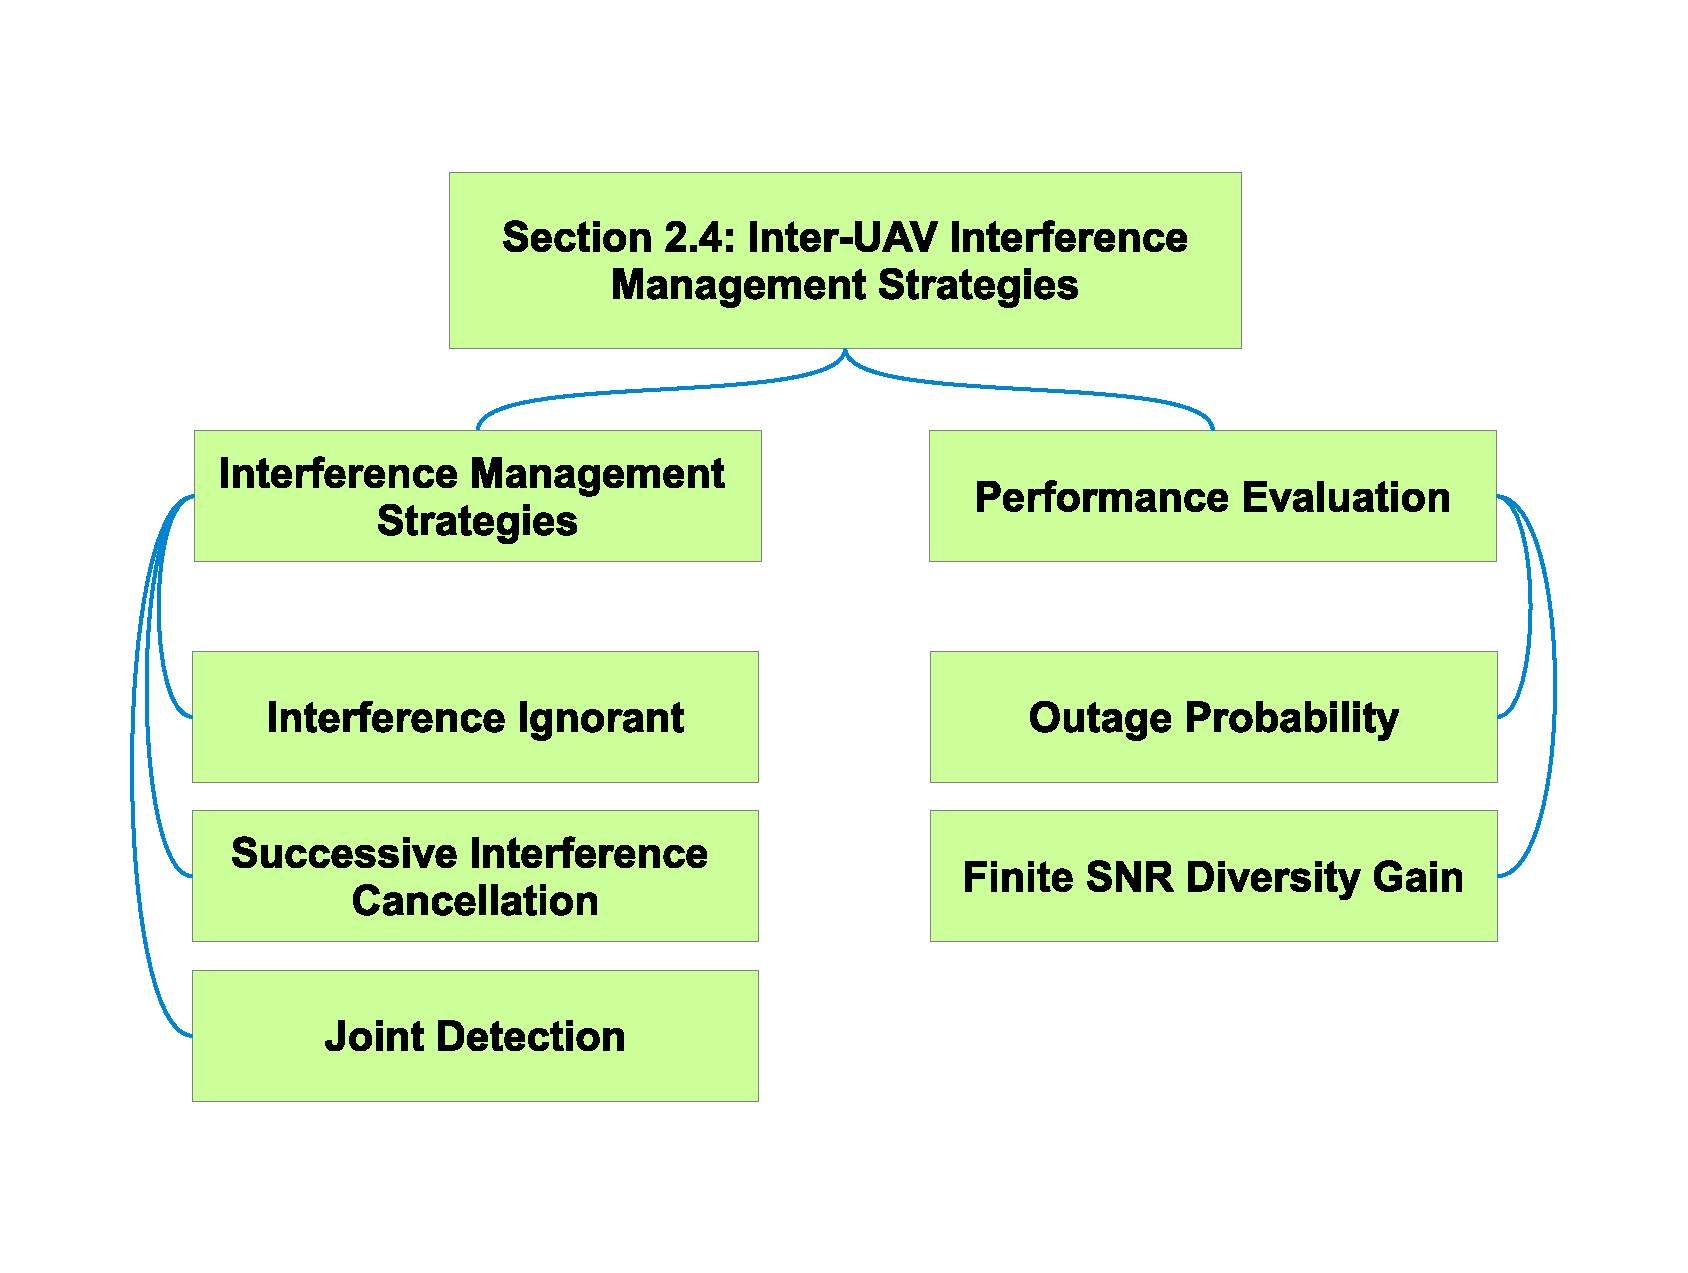
\includegraphics [width=0.7\columnwidth]{chap2_fig/sec_4_taxonomy.eps} 
\vspace{-0.5cm}
\caption{An overview of the topics in Section \ref{lit_review_sec_hd_uav_int}.}
%\vspace{-0.5cm}
\label{fig:lit_review_sec_4_taxonomy}
\end{figure}

\begin{figure} [h]
\centering
%\vspace{-1.5cm}
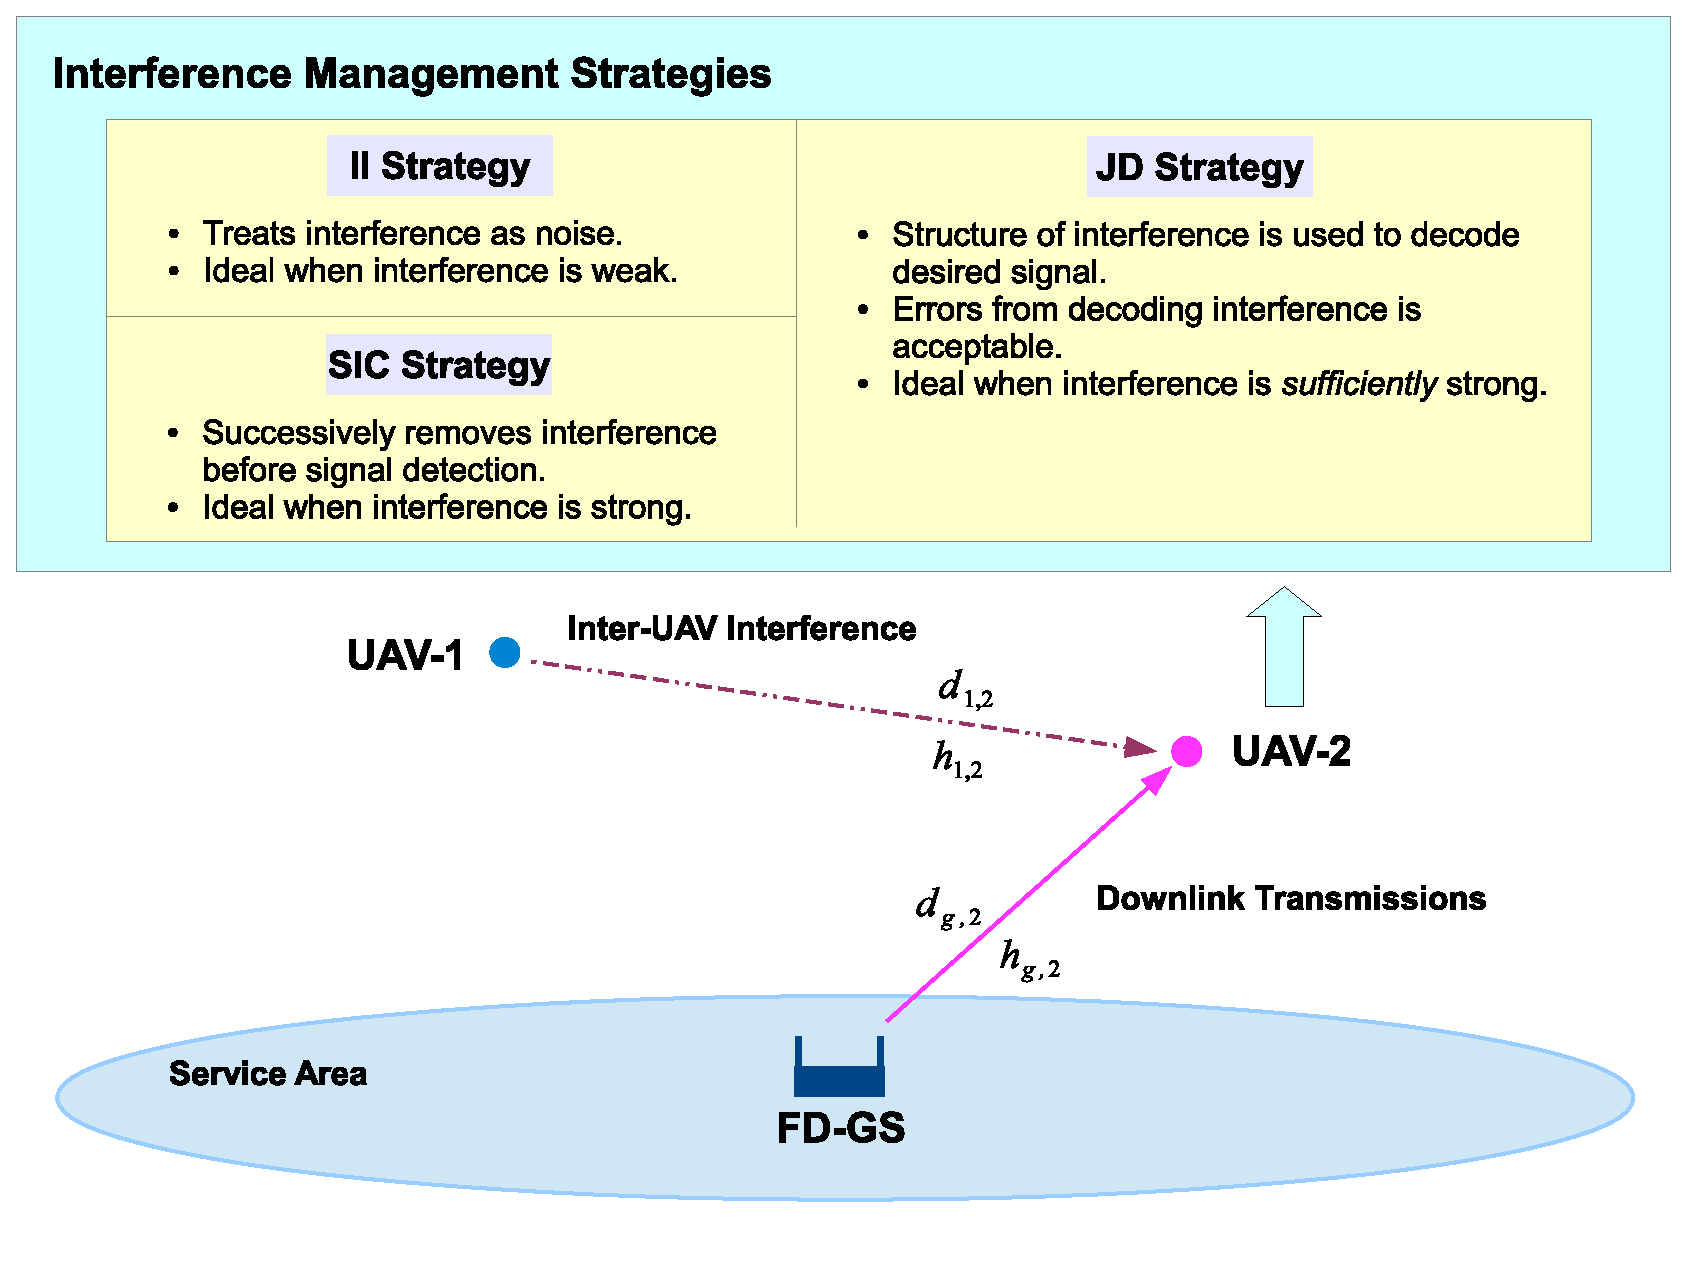
\includegraphics [width=0.6\columnwidth]{chap2_fig/interference_management_example.eps} 
%\vspace{-1.5cm}
\caption{An example of the types of interference management strategies that can be adopted for UAV-2 in the HBD-UCS.}
%\vspace{-0.5cm}
\label{fig:lit_review_interference_management_example}
\end{figure}

In HBD UAV communications, inter-UAV interference is experienced at the HD downlink UAVs due to simultaneous uplink and downlink transmissions. In this regard, a review of interference management techniques is presented in this section for HBD UAV communications. Thereafter, an overview of the performance analysis is presented for the discussed interference management techniques (Fig. \ref{fig:lit_review_interference_management_example}) for the HBD-UCS. An overview of the topics in this section is provided in Fig. \ref{fig:lit_review_sec_4_taxonomy}.

\subsection{Interference Management Strategies}
\begin{summary} \emph{
\emph{The II and SIC strategies offer effective inter-UAV interference management under weak and strong interference, respectively. However, inter-UAV interference management with JD, based on simultaneous non-unique decoding, outperforms both II and SIC strategies. 
}}
\end{summary}
As mentioned earlier, inter-UAV interference in HBD UAV communications is caused by uplink and downlink transmissions occurring concurrently on the same spectrum. With inter-UAV interference management being an important aspect of realizing HBD UAV communications, many interference management approaches have been investigated in the literature. Towards this endeavour, a review of interference management techniques for HBD UAV communications is presented below, with discussions focusing on the II, SIC, and JD approaches. A summary of studies on interference management strategies is also provided in Table \ref{table:lit_review_int_management_strategy}.

\subsubsection{Interference-Ignorant}
The II approach is a simple interference management strategy that ignores interference by treating it as noise \cite{ernest2019outage, tan2018joint, ernest2019power, etkin2008gaussian, sirigina2016symbol, sirigina2016full}. In weak interference scenarios, the II approach is sum rate optimal \cite{sirigina2016symbol}. However, under strong interference scenarios, the II approach is ineffective, particularly at high SNR regimes \cite{ernest2019outage}. Furthermore, since information can be obtained from the received interfering signals, an opportunity to exploit the underlying structure of the interference for interference management is lost in the II approach \cite{etkin2008gaussian}. 

Despite the limitations, the II approach has been analyzed for practical applications in wireless systems, e.g., in aeronautical communication systems \cite{ernest2019outage} and cellular networks \cite{sirigina2016full, bithas2015mobile}. For UAV communications, the II approach was investigated in \cite{tan2018ricianShad, tan2018joint, ernest2019power} for an HBD-UCS as depicted in Fig. \ref{fig:lit_review_interference_management_example}. Specifically, for the HBD-UCS in Fig. \ref{fig:lit_review_interference_management_example}, the II detector at UAV-2 treats the signal from the FD-enabled GS ($x_{gs}[t]$) as the SOI while treating the signal from UAV-1 ($x_1[t]$) as noise. Since the II approach is simple to implement, it can be used to provide effective interference management in an HBD-UCS for weak interference scenarios, as shown in \cite{tan2018joint, tan2018ricianShad}.

\subsubsection{Successive Interference Cancellation}
The SIC approach involves detecting and canceling the interference first, before the SOI is detected \cite{ernest2019outage, tan2018joint, ernest2019hybrid}. In particular, a SIC detector detects and removes the strongest interferer first, where the strongest interferer is defined either as the interferer with the highest average received power or the interfering node that is closest to the receiver \cite{weber2007transmission}. Doing so enables the SIC detector to remove the interferer with the highest signal-to-interference-plus-noise ratio (SINR) from the received composite signal \cite{weber2007transmission, qu2014understanding}. The SIC process is repeated until interference from nearby interfering nodes within a cancellation region around the receiver is removed \cite{weber2007transmission}, or interference is wholly removed from the received composite signal \cite{qu2014understanding}. For the former, the cancellation region describes a disk centered at the receiver, where a subset of the interfering nodes is located \cite{weber2007transmission}. The radius of the cancellation region is then chosen such that the interference cancellation for a specific average number of interfering nodes can be performed.

Additionally, the considered SIC process can be either perfect or imperfect. The perfect SIC model assumes that interference from the prior SIC stages is entirely removed, e.g., in \cite{ernest2019outage} and \cite{weber2007transmission}. For the case of imperfect SIC, residual interference from previously canceled interfering signals is considered at each stage of the SIC process, e.g., in \cite{weber2007transmission, ernest2019hybrid}. Putting the practical relevance of the imperfect SIC model into perspective, the residual interference can be used to account for non-ideal transmission conditions such as channel estimation errors.

In the literature, the SIC approach has been shown to improve the performance of interference-limited systems, e.g., in terms of reliability or transmission rate, for both perfect SIC \cite{ernest2019outage, tan2018joint, weber2007transmission, qu2014understanding} and imperfect SIC \cite{weber2007transmission, ernest2019hybrid}. Furthermore, it was shown in \cite{weber2007transmission} that through the cancellation of the strongest interferer alone, significant performance improvements can be obtained. However, for the SIC process to work, the transmission rate of each interferer must be constrained to meet the SINR requirement such that the strongest interferer transmits with the lowest rate, and so on \cite{qu2014understanding}. Therefore, enabling the SIC detector to support a large number of interfering nodes requires trading away the overall achievable rate, i.e., a tradeoff between SIC capability and achievable rate \cite{qu2014understanding}. 

Thus far, the SIC approach has attracted research interest, particularly in recent years, for various practical applications in wireless systems. For instance, the performance of SIC has been studied for cellular systems \cite{sirigina2016symbol, sirigina2016full, hasna2003performance, zhang2017full}. Likewise, the feasibility of the SIC approach has been studied for UAV communications in \cite{tan2018joint, ernest2019hybrid}. To illustrate, a two-stage SIC detector can be assumed for UAV-2 in Fig. \ref{fig:lit_review_interference_management_example}. The SIC detector at UAV-2 detects and removes $x_1[t]$ from UAV-1, before detecting the SOI $x_{gs}[t]$ from the FD-enabled GS. As shown in \cite{tan2018joint}, implementing SIC to manage inter-UAV interference enables the HBD-UCS to achieve better reliability over an equivalent HD-UCS in strong inter-UAV interference scenarios.

\begin{table*}[]
\centering
\caption{Summary of Studies on Interference Management Strategies}
\label{table:lit_review_int_management_strategy}
\scalebox{0.7}{
\begin{tabular}{llll}
\hline
Reference								& Approach					& Channel Model						& Performance Metric(s) 						\\ \hline \hline
\cite{ernest2019outage}	&	II, SIC						& Rician Fading						& Outage Probability, Finite SNR Diversity Gain, 	\\
												&										&													&	Finite SNR DMT 										\\
\cite{tan2018joint}			& II, SIC, JD (SND)	& Rician Fading						& Outage Probability, Finite SNR Diversity Gain,	\\
												&										&													&	Finite SNR DMT 										\\
\cite{ernest2019power}	& II, JD (SND) 			& Rician Fading, 					& Outage Probability 								\\
												&										& Rician Shadowed Fading	&																		\\
\cite{ernest2019hybrid}	& II, SIC			 			& Rician Fading						& Outage Probability 								\\
\cite{tan2018ricianShad}& II								& Rician Shadowed Fading 	& Outage Probability 								\\
\cite{sirigina2016full}	& II, JD (SND) 			& Rayleigh Fading					& Diversity Gain Region 						\\
\cite{bithas2015mobile}	&	II								& Rayleigh Fading, 				& Outage Probability, Average Bit Error Probability \\
												&										& Squared $K$-distribution \cite{abdi2001simple} &						\\
\cite{weber2007transmission}	& SIC					& Path Loss								& Outage Probability, Transmission Capacity \\
\cite{qu2014understanding}		& SIC					& Rayleigh Fading					& Throughput, CPU Run Time 					\\
\cite{bidokhti2014non} 	&	JD (SD, SND)			& - 											& Rate Region 											\\
\cite{nam2014advanced} 	& II, JD (SD, SND) 	& Static AWGN 						& Rate Region, Throughput 					\\
\cite{zhou2015mac} 			& JD (SD) 					& Path Loss							 	& Capacity Region \\
\cite{bandemer2012simultaneous} & JD (SND) 	& - 											& Rate Region \\
\cite{kim2019off} 			&	JD (SND) 					& Rayleigh Fading 				& Asymptotic DMT  \\ \hline
\end{tabular}}
\end{table*}

\subsubsection{Joint Detection}
The JD approach involves the joint detection of the SOI and interfering signals during the detection process. In the literature, multiple JD approaches have been studied. Of particular importance are two types of JD techniques, namely simultaneous decoding (SD) \cite{bidokhti2014non, nam2014advanced, zhou2015mac} and simultaneous non-unique decoding (SND) \cite{bidokhti2014non, nam2014advanced, bandemer2012simultaneous}.\footnote{In \cite{bidokhti2014non}, SD and SND are referred as joint unique decoding and non-unique decoding, respectively.} In SD, the receiver employs a strategy that utilizes the underlying structure of the interference to decode correctly, i.e., detect, both SOI and interference signal \cite{bidokhti2014non, nam2014advanced, zhou2015mac, bandemer2012simultaneous}.

In contrast, SND employs a strategy that is similar to SD, except that errors from decoding, i.e., detecting, the interfering signals are tolerated \cite{bidokhti2014non, nam2014advanced, bandemer2012simultaneous}. Thus, the SND strategy only focuses on the correct detection of the SOI transmitted over the interference channel. As it turns out, the SND strategy can attain the rate regions of the SD strategy and the II approach \cite{nam2014advanced, bandemer2012simultaneous}. As such, when compared to SD, SND attains better performance by simultaneously achieving the combined rate regions of the SD and the II approaches \cite{nam2014advanced, bandemer2012simultaneous}, albeit at the cost of high complexity \cite{tan2018joint}. In light of the benefits brought on by the SND strategy, in the remainder of this section, discussions on JD will henceforth refer to the SND strategy.

It is noted that the JD approach, i.e., SND strategy, has been investigated for potential applications in practical wireless systems. For instance, a 2-user multiple input multiple output (MIMO) system was proposed in \cite{kim2019off} that combines transmissions using interference alignment, i.e., beamforming, with receivers that adopt JD. For UAV communications, the feasibility of JD was studied in \cite{tan2018joint}. In particular, a joint detector employing the SND strategy can be equipped on UAV-2 for the HBD-UCS depicted in Fig. \ref{fig:lit_review_interference_management_example}. Thereafter, the joint detector at UAV-2 jointly detects $x_{gs}[t]$ and $x_1[t]$ from the FD-enabled GS and UAV-1, respectively. Following the principles of the SND strategy, detection errors of the interfering signal $x_1[t]$ are tolerated by the joint detector at UAV-2, since the focus is on detecting the SOI $x_{gs}[t]$. Extensive performance analysis of a JD-based HBD-UCS in \cite{tan2018joint} has demonstrated that the JD approach outperforms the II and SIC approaches. In particular, the JD approach enables the HBD-UCS to achieve higher reliability than the II and SIC approaches while supporting a wider range of QoS requirements. Thus, JD is the most attractive interference management technique for HBD UAV communications when compared against the II, and SIC approaches.

\subsection{Performance Evaluation of the II, SIC, and JD Strategies for HBD UAV Communications}
\begin{summary} \emph{
\emph{Outage probability and finite SNR diversity gain are useful tools in determining the effectiveness of the II, SIC, and JD approaches for inter-UAV interference management. In this aspect, JD attains lower outage probability and higher finite SNR diversity gain than the II and SIC approach.
}}
\end{summary}

In this subsection, a review of the performance analysis of the II, SIC, and JD approaches is presented. To show the effectiveness of the considered interference management strategies for HBD UAV communications, the outage probability and finite SNR diversity gain of the II, SIC, and JD approaches are also discussed in the context of the HBD-UCS depicted in Fig. \ref{fig:lit_review_interference_management_example}. 

\begin{figure*}[]
\centering
\subfloat[II Approach]{\includegraphics [width=0.49\columnwidth]{chap2_fig/II_interference_management_example.eps} 
\label{fig:lit_review_II_rate_regions}}
\hfil
\subfloat[SIC Approach]{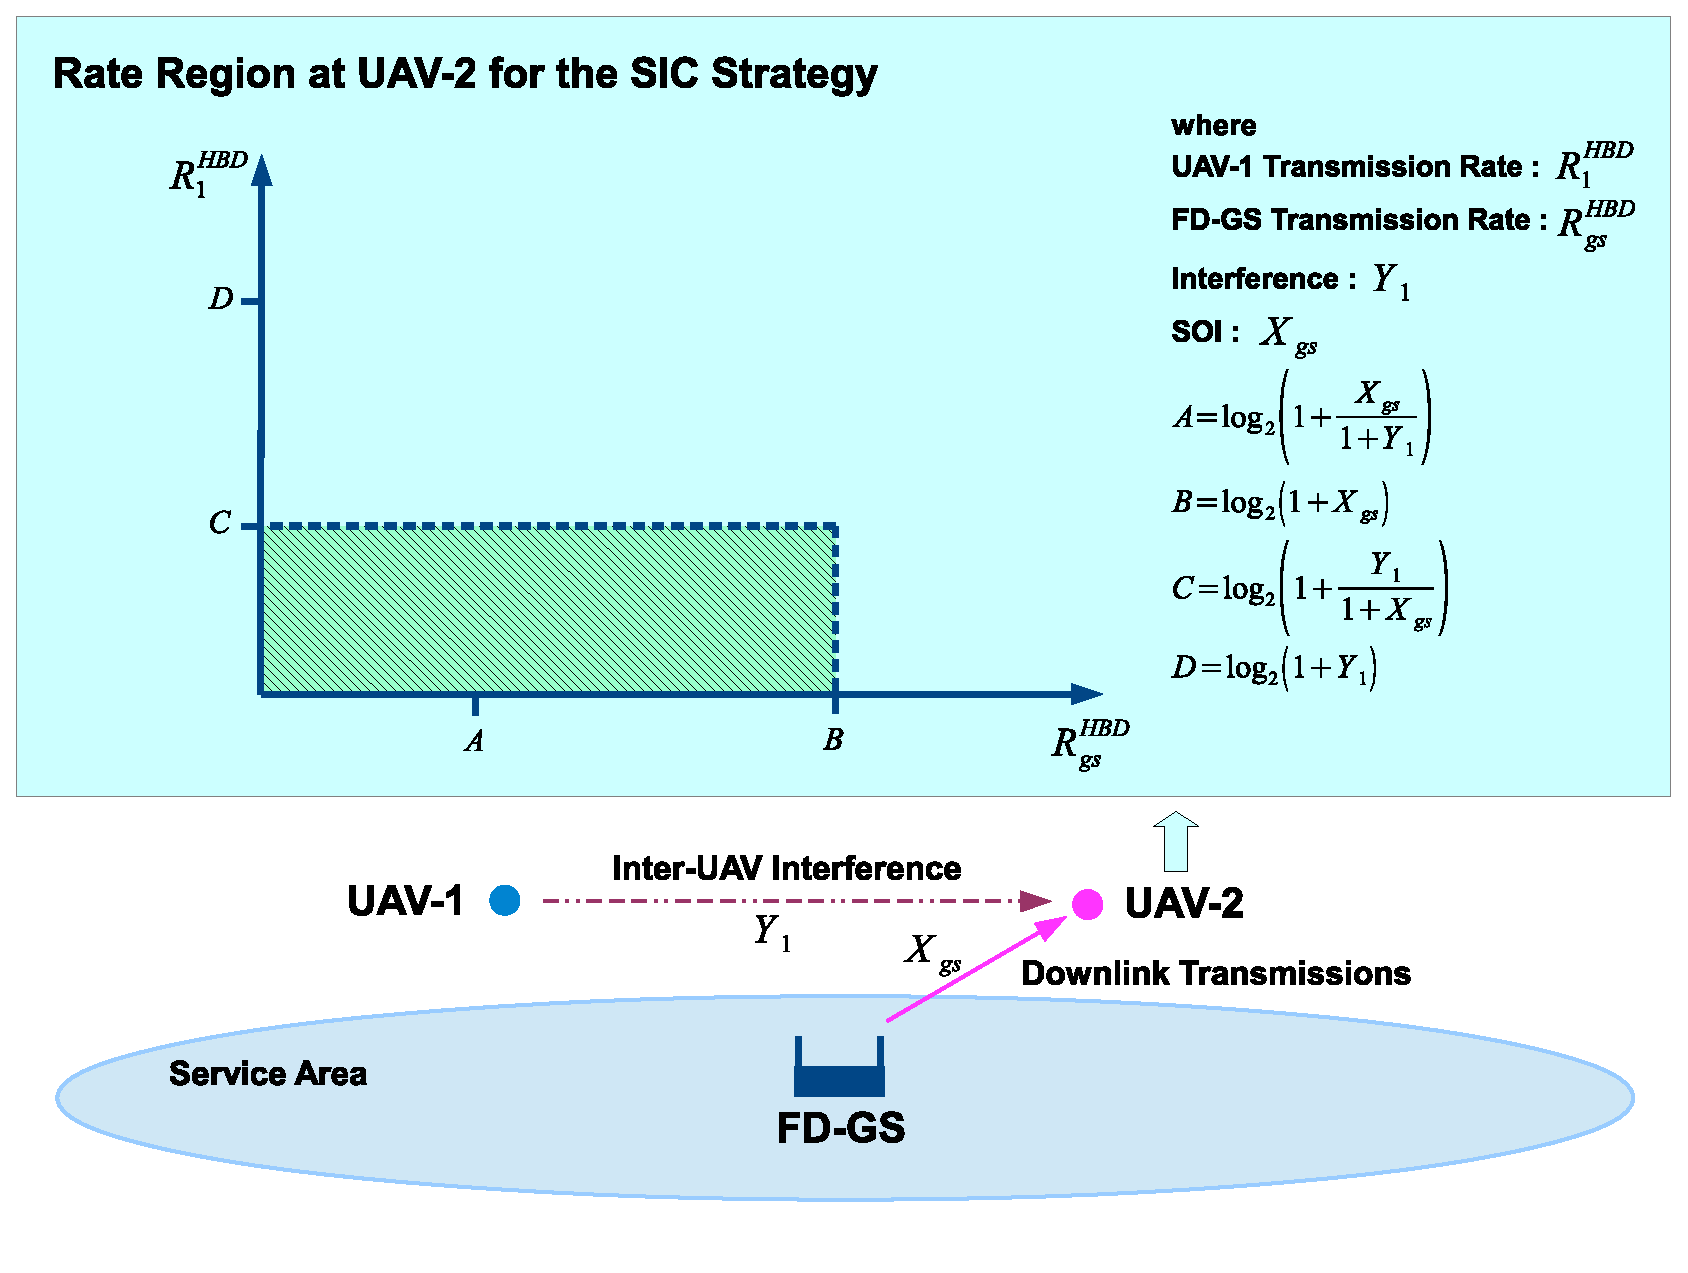
\includegraphics [width=0.49\columnwidth]{chap2_fig/SIC_interference_management_example.eps} 
\label{fig:lit_review_SIC_rate_regions}}
\hfil
\subfloat[JD Approach]{\includegraphics [width=0.49\columnwidth]{chap2_fig/JD_interference_management_example.eps} 
\label{fig:lit_review_JD_rate_regions}}
\caption{The achievable instantaneous rate region of the II, SIC, and JD interference management approaches. The transmission rate of the FD-GS and UAV-1 are denoted as $R_{GS}^{HBD}$ and $R_{1}^{HBD}$, respectively. The variables $X_{gs}$ and $Y_1$ denote the SOI and interference at UAV-2, respectively.}
\label{fig:lit_review_rate_regions}
\end{figure*}

\subsubsection{Outage Probability}
One way to gauge the feasibility of the II, SIC, and JD approaches is to analyze the reliability of HBD UAV communications. In this sense, outage probability is a useful metric as it can be used to represent the packet error rate ($PER$) of the HBD-UCS for transmissions spanning over one fading block \cite{ernest2019outage, lin2013outage}, i.e., block fading assumption. 

To obtain any meaningful analysis, closed-form outage probability expressions that can accurately reflect the communications environment, e.g., small-scale fading, receiver noise, and interference, are needed for the II, SIC, and JD approaches. For instance, closed-form outage probability expressions for the II detector are available for transmissions over Nakagami-$m$ fading channels \cite{yao1992investigations}, and composite fading scenarios, where the SOI is transmitted over Rayleigh fading channels and interference is experienced over squared ${\mathcal{K}}$-distributed channels \cite{bithas2015mobile}. More recently, a unified moment-based approach was proposed by Rached et al. \cite{rached2017unified} that presents closed-form outage probability expressions for transmissions over various types of fading channels, including Rician fading channels that are encountered in UAV communications. Based on the work in \cite{rached2017unified}, the II detector was subsequently analyzed for HBD-based aeronautical communication systems \cite{ernest2019outage,ernest2018performance} and HBD-UCSs over Rician fading channels \cite{tan2018ricianShad, tan2018joint, ernest2018hybrid, ernest2019power, ernest2019hybrid} and Rician shadowed fading channels \cite{ernest2019noma,ernest2019power}.

Similarly, closed-form outage probability expressions for SIC detectors are available in \cite{hasna2003performance} and \cite{romero2008receive}. In particular, the analysis in \cite{hasna2003performance} and \cite{romero2008receive} assumes that the SOI is transmitted either over Nakagami-$m$, Rayleigh, or Rician fading channels while interference is experienced over Rayleigh fading channels. However, the resultant closed-form expressions presented in \cite{hasna2003performance} and \cite{romero2008receive} are for partial SIC, where there is at least one remaining interferer once the SIC process ends. In \cite{zhang2017full}, closed-form outage probability expressions were derived for a two-stage SIC detector that receives power-domain NOMA transmissions over Rayleigh fading channels. Apart from the studies mentioned above, closed-form outage probability expressions for a two-stage SIC detector was derived in \cite{ernest2019outage} for an HBD aeronautical communication system, and also in \cite{tan2018joint, ernest2018hybrid} for an HBD-UCS, where both the SOI and interference are transmitted over Rician fading channels.

For the case of the JD approach, closed-form outage probability expressions have been presented in \cite{elkourdi2011femtocell} and \cite{wui2016outage} for receivers operating in a Rayleigh fading environment. In particular, the analysis in \cite{elkourdi2011femtocell} and \cite{wui2016outage} was conducted for femtocell relay systems and cognitive radio systems, respectively, where the SND strategy was assumed at the relay node. In \cite{tan2018joint}, closed-form outage probability expressions for JD in an HBD-UCS was derived over Rician fading channels, where it was shown that JD achieves near-optimal outage probability.

\begin{table*}[t]
\centering
\caption{Outage probability definitions of the II, SIC, and joint detectors at UAV-2.}
\label{table:lit_review_ref_schemes_outage}
\scalebox{0.7}{
\begin{tabular}{llll}
\hline
Protocol/Detector 			& Outage Notation	& Outage Event Definitions	& References  \\ \hline \hline \vspace{0.05cm}
II Detector 						& $Pr\big(\mathcal{O}_{2}^{HBD(II)}\big)$ 	& $\mathcal{O}_{2}^{HBD(II)}  = \Big\{ h_{g,2}, h_{1,2} : R_{gs}^{HBD} \geq \log_{2}\Big(1+\frac{X_{gs}}{Y_{1} + 1}\Big)\Big\}$ & \cite[eq. (7)]{ernest2019outage} \\ \vspace{0.05cm}
SIC Detector 						& $Pr\big(\mathcal{O}_{2}^{HBD(SIC)}\big)$	& $\mathcal{O}_{2}^{HBD(SIC)} = \bigg\{h_{g,2}, h_{1,2} : R_{1}^{HBD} > \log_{2}\bigg(1+\frac{Y_{1}}{1+X_{gs}}\bigg) \bigg\}$ 	&	\cite[eq. (9)]{ernest2019outage}  \\ \vspace{0.05cm}
												&																						& $\cup \bigg\{h_{g,2}, h_{1,2} :  R_{1}^{HBD} \leq \log_{2}\bigg(1+\frac{Y_{1}}{1+X_{gs}}\bigg), R_{gs}^{HBD} > \log_{2}\big(1+X_{gs}\big) \bigg\}_.$				&		 \\ \vspace{0.05cm}
Joint Detector 					& $Pr\big(\mathcal{O}_{2}^{HBD(JD)}\big)$ 	& $\mathcal{O}_{2}^{HBD(JD)} = \mathcal{O}_{JD}^{1} \cup \mathcal{O}_{JD}^{2}$ 																									& \cite[eq. (9)]{tan2018joint} \\ \vspace{0.05cm}
												&																						&	$\mathcal{O}_{JD}^{1} = \bigg\{h_{g,2}, h_{1,2} : R_{gs}^{HBD} > \log_{2}\bigg(1+X_{gs}\bigg)\bigg\}$													& \\ \vspace{0.05cm}
												& 																					& $\mathcal{O}_{JD}^{2} = \bigg\{h_{g,2}, h_{1,2} : R_{1}^{HBD} + R_{gs}^{HBD} > \log_{2}\bigg(1+X_{gs}+Y_{1} \bigg)_,$					& \\ \vspace{0.05cm}
												&																						& $\hspace{1.2cm} \log_{2}\bigg(1+\frac{X_{gs}}{1+Y_{1}} \bigg) \leq R_{gs}^{HBD} \leq \log_{2}\bigg(1+X_{gs}\bigg) \bigg\}$		& \\ \vspace{0.05cm}
HD-UCS 									& $Pr\big(\mathcal{O}_{2}^{HD}\big)$ 				& $\mathcal{O}_{2}^{HD}  = \Big\{ h_{g,2} : R_{gs}^{HD} \geq \log_{2}\Big(1+X_{gs}\Big)\Big\}$																	&	\cite[eq. (11)]{ernest2019outage}  \\ \hline
\end{tabular}}
\end{table*}

From the above discussions, the outage probability of the II, SIC, and JD approaches has been well analyzed for an HBD-UCS (Fig. \ref{fig:lit_review_interference_management_example}), each with different advantages and limitations. To better illustrate this, the achievable instantaneous rate regions of the II, SIC and JD approaches at UAV-2 are depicted in Fig. \ref{fig:lit_review_rate_regions} \cite[Fig. 2]{tan2018joint}, where $X_{gs}$ and $Y_{1}$ denote the SOI from the FD-GS and interference from UAV-1, respectively. From Fig. \ref{fig:lit_review_rate_regions}, it is evident that JD achieves the largest achievable instantaneous rate region (Fig. \ref{fig:lit_review_JD_rate_regions}) compared to the II (Fig. \ref{fig:lit_review_II_rate_regions}) and SIC (Fig. \ref{fig:lit_review_SIC_rate_regions}) approaches at the cost of higher complexity costs \cite{tan2018joint}. Consequently, JD exhibits the smallest outage region when compared to the II and SIC detectors. 

Based on the achievable instantaneous rate regions in Fig. \ref{fig:lit_review_rate_regions} \cite[Fig. 2]{tan2018joint}, the resulting outage events, closed-form outage probability expressions, and the associated references are given in Table \ref{table:lit_review_ref_schemes_outage}. The outage probability of the II, SIC, and joint detectors was analyzed in \cite[Fig. 3]{tan2018joint}, where it is noted that the JD approach attains ideal, i.e., interference-free, outage probability under sufficiently strong inter-UAV interference and is not interference-limited at high SNR regimes. In contrast, the II and SIC detectors only work well under weak and strong inter-UAV interference, respectively, and are interference-limited at high SNR regimes \cite{tan2018joint}. Thus, the effectiveness and suitability of adopting JD to manage inter-UAV interference are demonstrated.

\subsubsection{Finite SNR Diversity Gain}
Finite SNR diversity gain is another metric of interest which quantifies the outage probability decay of a given system operating at a particular SNR, with fixed transmission rate \cite{shin2008diversity}. When variable transmission rates are considered, then one can also analyze the finite SNR DMT by varying the transmission rate, i.e., multiplexing gain, to gauge the finite SNR diversity gain \cite{narasimhan2006finite}. In particular, for a wireless system with \textcolor{black}{instantaneous channel gain $\mathcal{H}$, outage event $\mathcal{O} = \{\mathcal{H}<\gamma\}$}, outage probability $Pr\big(\mathcal{O}\big)$, transmission rate $R$, threshold $\gamma = 2^R - 1$, and normalized average received power $\Omega$, the asymptotic SNR diversity gain $d$ is \cite{zheng2003diversity}:
%%%%%%%%%%%%%%%%%%%%%%%%%%%%%%%%%%%%%%%%%%%%%%%%%%%%%%%%%%%%%%%%%%%%%%%%%%%%%%%%%
\begin{eqnarray} \label{lit_review_asymp_diversity_gain}
 d = \lim_{\Omega\to\infty} \frac{\log_2(Pr\big(\mathcal{O}\big))}{\log_2(\Omega)}_.
\end{eqnarray}
%%%%%%%%%%%%%%%%%%%%%%%%%%%%%%%%%%%%%%%%%%%%%%%%%%%%%%%%%%%%%%%%%%%%%%%%%%%%%%%%%

At finite SNR regimes, i.e., low-to-moderate SNRs, the finite SNR diversity gain $d_f$ is \cite[Eq. (5)]{narasimhan2006finite}:
%%%%%%%%%%%%%%%%%%%%%%%%%%%%%%%%%%%%%%%%%%%%%%%%%%%%%%%%%%%%%%%%%%%%%%%%%%%%%%%%%
\begin{eqnarray} \label{lit_review_df}
d_f = \frac{-\Omega}{Pr\big(\mathcal{O}\big)}\frac{\partial}{\partial\Omega}Pr\big(\mathcal{O}\big)_,
\end{eqnarray}
%%%%%%%%%%%%%%%%%%%%%%%%%%%%%%%%%%%%%%%%%%%%%%%%%%%%%%%%%%%%%%%%%%%%%%%%%%%%%%%%%
where $\lim_{\Omega\to\infty}d_f = d$ \cite{shin2008diversity, heidarpour2017finite} and is consistent with (\ref{lit_review_asymp_diversity_gain}) when evaluated at asymptotic SNR regimes \cite{zheng2003diversity}. Furthermore, when the transmission rate varies depending on $\Omega$, i.e., variable transmission rate, the asymptotic SNR multiplexing gain $r$ is modeled as \cite{zheng2003diversity}:
%%%%%%%%%%%%%%%%%%%%%%%%%%%%%%%%%%%%%%%%%%%%%%%%%%%%%%%%%%%%%%%%%%%%%%%%%%%%%%%%%
\begin{eqnarray} \label{lit_review_asymp_mult_gain}
r = \lim_{\Omega\to\infty} \frac{R(\Omega)}{\log_2(\Omega)}
\end{eqnarray}
%%%%%%%%%%%%%%%%%%%%%%%%%%%%%%%%%%%%%%%%%%%%%%%%%%%%%%%%%%%%%%%%%%%%%%%%%%%%%%%%%
and, accordingly, the finite SNR multiplexing gain $r_f$ is given as \cite[Eq. (4)]{narasimhan2006finite}:
%%%%%%%%%%%%%%%%%%%%%%%%%%%%%%%%%%%%%%%%%%%%%%%%%%%%%%%%%%%%%%%%%%%%%%%%%%%%%%%%%
\begin{eqnarray} \label{lit_review_rf}
r_f = \frac{R(\Omega)}{\log_2(1+\Omega)}_.
\end{eqnarray}
%%%%%%%%%%%%%%%%%%%%%%%%%%%%%%%%%%%%%%%%%%%%%%%%%%%%%%%%%%%%%%%%%%%%%%%%%%%%%%%%%

Through finite SNR diversity gain and finite SNR DMT analysis, outage deviation behaviors, which will otherwise not be present at asymptotically high SNRs due to small-scale fading, are revealed \cite{shin2008diversity}. In terms of practical relevance, finite SNR diversity gain analysis can be used to characterize the outage probability performance of wireless systems, which are typically designed to operate at low-to-moderate SNR ranges \cite{ernest2019outage}. Furthermore, finite SNR diversity gain can be used to estimate the required SNR before a targeted rate of error decay is achieved \cite{narasimhan2006finite}, e.g., via turbo codes or low-density parity-check codes. Moreover, when outage probability is analyzed in conjunction with finite SNR diversity gain, one obtains the upper and lower limits of a system's bit error rate performance \cite{ernest2019outage, zheng2003diversity, nabar2005diversity}. 

In the literature, several studies have analyzed finite SNR diversity gain over Nakagami-$m$ fading channels \cite{wang2012finite} and Rayleigh fading channels \cite{lin2013outage,yang2015efficient}. For Rician fading channels, Shin et al. \cite{shin2008diversity} and      Narasimhan \cite{narasimhan2006finite} characterized the finite SNR diversity gain and finite SNR DMT for MIMO systems, where the impact of Rician $K$ factors on outage behavior and finite SNR DMT was noted. The analysis of finite SNR diversity gain and finite SNR DMT has also been applied to several other wireless systems. In \cite{heidarpour2017finite}, finite SNR DMT analysis was analyzed for a network coded cooperative communication system. Despite the above studies, the literature discussing the application of finite SNR analysis in practical wireless systems is still limited, particularly for UAV communications. For instance, only the application of DMT analysis, i.e., diversity gain at asymptotic SNR regimes, for cellular systems was studied in \cite{sirigina2016symbol, sirigina2016full}, where the SIC approach was considered. Likewise, in \cite{kim2019off} where the II and the JD approach was considered, the authors focused only on DMT analysis. 

\begin{table*}[t]
\centering
\caption{References of finite SNR diversity gain and finite SNR DMT expressions for the II, SIC, and joint detectors at UAV-2.}
\label{table:lit_review_ref_schemes_diversity_gain}
\scalebox{0.7}{
\begin{tabular}{lllll}
\hline
Protocol/Detector 			& Finite SNR  							& Finite SNR 		& References (Diversity Gain) & References (DMT)  \\
												&	Diversity Gain Notation		&	DMT Notation	&															&										\\ \hline \hline \vspace{0.05cm}
II Detector 						& $d_{f,2}^{HBD(II)}$									& $d_{f,2}^{HBD(II)*}$		& \cite[eq. (21)]{ernest2019outage} & \cite[eq. (22)]{tan2018joint} \\ \vspace{0.05cm}
SIC Detector 						& $d_{f,2}^{HBD(SIC)}$								& $d_{f,2}^{HBD(SIC)*}$		&	\cite[eq. (22)]{ernest2019outage} & \cite[eq. (23)]{tan2018joint} \\ \vspace{0.05cm}
Joint Detector 					&	$d_{f,2}^{HBD(JD)}$								 	& $d_{f,2}^{HBD(JD)*}$		& \cite[eq. (18)]{tan2018joint}			& \cite[eq. (24)]{tan2018joint} \\ \vspace{0.05cm}
HD-UCS 									& $d_{f,2}^{HD}$											&	$d_{f,2}^{HD*}$					&	\cite[eq. (25)]{ernest2019outage} & \cite[eq. (31)]{ernest2019outage} \\ \hline
\end{tabular}}
\end{table*}

To this end, closed-form expressions for the finite SNR diversity gain and finite SNR DMT of the II and SIC approaches were presented in \cite{ernest2019outage} for aeronautical communication systems. Similarly, in \cite{tan2018joint}, closed-form expressions were presented for the finite SNR diversity gain and finite SNR DMT of a joint detector at UAV-2. In both \cite{ernest2019outage} and \cite{tan2018joint}, the resulting finite SNR analysis yielded closed-form expressions, which are summarized in Table \ref{table:lit_review_ref_schemes_diversity_gain}. 

From \cite[Fig. 3]{tan2018joint} and \cite[Fig. 5]{tan2018joint}, it is noted that the II and SIC detectors achieve non-zero diversity gain at low SNR regimes under weak and strong inter-UAV interference, respectively. Also, at high SNR regimes, both the II and SIC detectors achieve zero diversity gain and are thus interference-limited. In contrast, the joint detector achieves ideal, i.e., interference-free, diversity gain when inter-UAV interference is sufficiently strong. Furthermore, the joint detector attains a diversity gain of one at high SNR regimes and is, therefore, not interference-limited. Through finite SNR analysis, the superiority of the JD approach for inter-UAV interference management over the II and SIC approaches is demonstrated. Furthermore, the use of finite SNR diversity gain as a useful tool to identify scenarios where the HBD-UCS becomes interference-limited is highlighted.

%%%%%%%%%%%%%%%%%%%%%%%%%%%%%%%%%%%%%%%%%%%%%%%%%%%%%%%%%%%%%%%%%%%%%%%%%%%%%%%%%%%%%%%%%%%%%%%%%%%%%%%%%%%%%%%%%%%%%%%%%%%%%%%%%%%%%%%%%
% Section: NOMA
\section{Power-Domain Non-Orthogonal Multiple Access for HBD UAV Communications} \label{lit_review_sec_noma}

\begin{figure} [tpb]
\centering
%\vspace{-1cm}
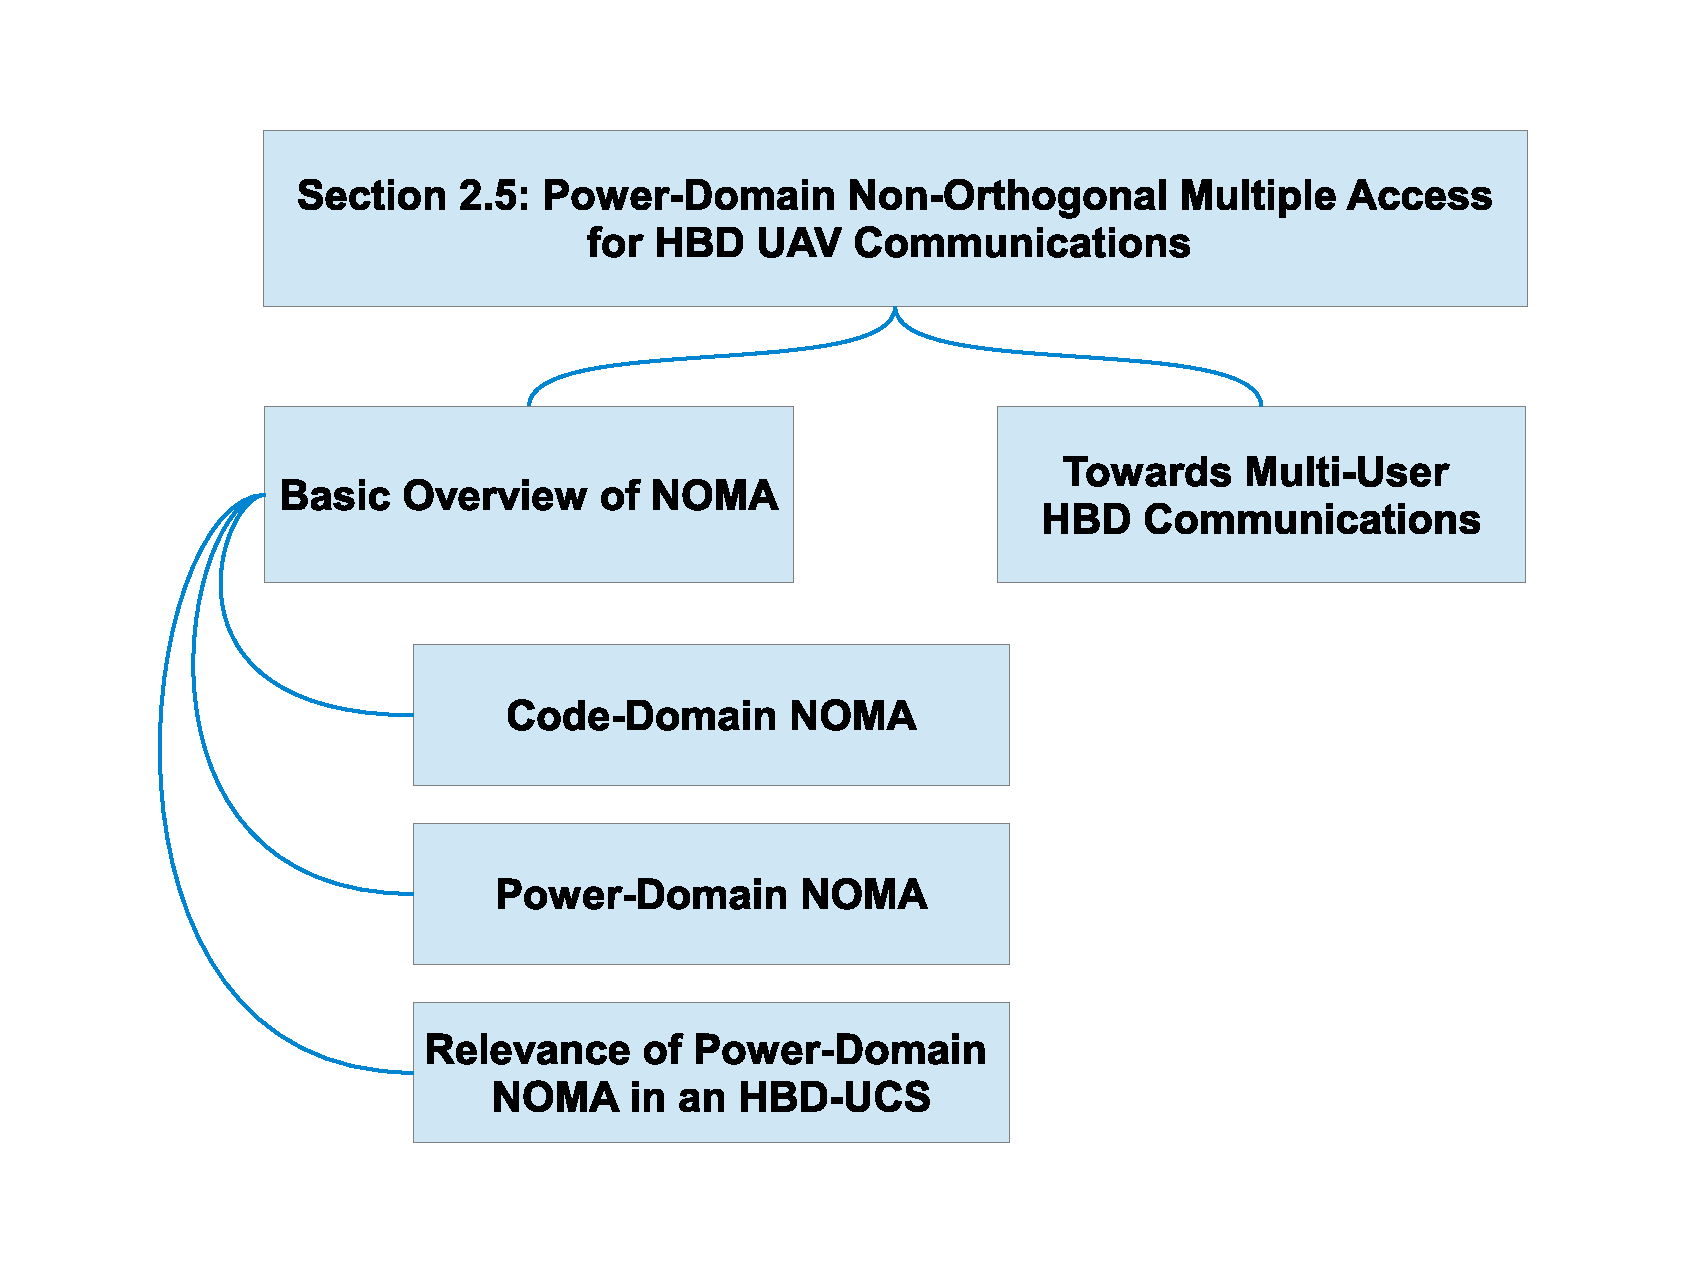
\includegraphics [width=0.7\columnwidth]{chap2_fig/sec_5_taxonomy.eps} 
\vspace{-0.5cm}
\caption{An overview of the topics in Section \ref{lit_review_sec_noma}.}
%\vspace{-0.5cm}
\label{fig:lit_review_sec_5_taxonomy}
\end{figure}

%%%%%%%%%%%%%%%%%%%%%%%%%%%%%%%%%%%%%%%%%%%%%%%%%%%%%%%%%%%%%%%%%%%%%%%%%%%%%%%%%%%%%%%%%%%%%%%%%%%%%%%%%%%%%%%%%%%%%%%%%%%%%%%%%%%%%%%%%
%Discussions of the HBD-UCS has thus far been conducted under the assumption of one uplink UAV and one downlink UAV in the system model, e.g., Fig. \ref{fig:block_diagram}. When an arbitrary number of uplink and downlink UAVs is considered in the system model, how the UAVs and FD-enabled GS transmit and receive messages will also change. In particular, to adhere to HBD transmission principles, the FD-enabled GS concurrently receives messages from all uplink UAVs while broadcasting messages to the downlink UAVs on the same spectrum. To enable the recovery of messages at the FD-enabled GS and downlink UAVs, one can adopt power-domain non-orthogonal multiple access (NOMA) in the HBD-UCS. In this regard, discussions pertaining to preliminary NOMA concepts and enabling methods to implement power-domain NOMA in an HBD-UCS are presented in this section. Thereafter, the associated open research problems and challenges of employing power-domain NOMA in HBD UAV communications are discussed.
%%%%%%%%%%%%%%%%%%%%%%%%%%%%%%%%%%%%%%%%%%%%%%%%%%%%%%%%%%%%%%%%%%%%%%%%%%%%%%%%%%%%%%%%%%%%%%%%%%%%%%%%%%%%%%%%%%%%%%%%%%%%%%%%%%%%%%%%%

Discussions of the HBD-UCS has thus far been conducted under the assumption of one uplink UAV and one downlink UAV in the system model, e.g., Fig. \ref{fig:lit_review_interference_management_example}. When an arbitrary number of uplink and downlink UAVs is considered in the system model, \textcolor{black}{approaches that enable an accurate representation of UAV deployments and multi-UAV communications are needed. One such approach that can be considered is stochastic geometry. Specifically, stochastic geometry has been extensively employed in cellular networks, where the locations of base stations and user equipments are modeled as Poisson point processes (PPPs). However, in the context of multi-UAV networks, recent works, e.g., \cite{chetlur2017downlink} and \cite{wang2018modeling} have shown binomial point processes (BPPs) to be more suitable due to the fixed number of deployed nodes in such networks.}

\textcolor{black}{Apart from UAV deployments,} the detection of the desired messages at the UAVs and FD-enabled GS is also changed. In particular, to adhere to HBD transmission principles, the FD-enabled GS concurrently receives messages from all uplink UAVs while broadcasting messages to the downlink UAVs on the same spectrum. In this regard, discussions of multi-user HBD systems, preliminary NOMA concepts, and enabling methods to implement power-domain NOMA in an HBD-UCS are presented in the rest of this section. An overview of the topics in this section is provided in Fig. \ref{fig:lit_review_sec_5_taxonomy}.

\subsection{Towards Multi-User HBD Communications}

\begin{summary}
\emph{
\emph{While multi-user HBD communications can be implemented through FD systems based on TDMA, OFDMA, or CDMA, spectrum efficiency improvement is still limited due to constraints on the number of users sharing each time-frequency resources, interference, and computational complexity.}
}
\end{summary}

For the recovery of messages at the FD-enabled GS and downlink UAVs, groups of uplink and downlink UAVs can be scheduled to share the same time-frequency resource blocks. Notably, in such multi-user FD-based systems, uplink and downlink nodes can be scheduled to share the same time-frequency resource block via time division multiple access (TDMA) or orthogonal frequency division multiple access (OFDMA) \cite{wang2015exploiting}. 

\textcolor{black}{For sharing of time-frequency resource blocks in time domain}, TDMA-based FD systems have been noted in energy harvesting (EH) communication systems such as FD wireless powered communication networks (FD-WPCNs) \cite{ju2014optimal, kang2015full} and FD ambient backscatter communication networks (FD-ABCNs) \cite{yang2019optimal}. In FD-WPCNs, energy and information transmission co-occur over the same time slot and spectrum \cite{ju2014optimal, kang2015full}. For a frame with $K+1$ time slots, frame duration $T$, and time slot duration $\tau_iT, i \in \{0, K\}$, an FD access point (FD-AP) transmits energy to all HD downlink EH users throughout the frame duration $T$. Also, TDMA is employed to receive information from EH users. Specifically, the FD-AP receives uplink data from the HD EH user-$i$ at the $i$th time slot while concurrently transmitting energy over the same spectrum. For FD-ABCNs, an FD-AP transmits messages to a legacy user (LU) throughout the frame duration ($T$) \cite{yang2019optimal}. Concurrently, at the HD EH backscatter devices (BD), the received ambient messages are modulated and reflected back to the FD-AP. Similar to FD-WPCNs, TDMA is employed to schedule the BD uplink transmissions \cite{yang2019optimal}. Thus, BD-$i$ transmits information to the FD-AP at the $i$th time slot while the FD-AP is simultaneously transmitting messages to the LU on the same spectrum. For the latter, OFMDA FD systems have been investigated in cellular systems to improve spectrum efficiency \cite{shao2014analysis,nam2015joint,di2016joint,zhang2019max}. In such OFDMA cellular systems, each subcarrier supports one uplink user and one downlink user. Doing so allows an FD base station to transmit messages to the downlink user while concurrently receiving information from the uplink user. Apart from TDMA-based and OFDMA FD systems, multi-user FD-based systems can also enable the sharing of the same time-frequency resource block in code domain through code-division multiple access (CDMA) \cite{chen2015physical}. For instance, in \cite{gao2014full}, CDMA was employed as the multiple access scheme for a multi-user system with an FD relay. 

Evidently, for TDMA-based and OFDMA FD systems, the improvement to spectrum efficiency is limited as only one pair of uplink and downlink user can utilize the same time-frequency resource block at any time instant. The limit of one uplink and downlink user pair per resource block stems from the need to avoid uplink interference at the downlink user, e.g., at the EH user in FD-WPCN \cite{kang2015full} and downlink user in OFDMA FD cellular systems \cite{zhang2019max}. For CDMA-based FD-systems, spectrum efficiency comes at the cost of SI, interference due to CDMA code correlation, and computational complexity. Yet, it is important to note that the recent advances in interference mitigation techniques, e.g., SIC, have demonstrated the feasibility of allowing more users to share the same time-frequency resource in FD systems.

Therefore, one may wish to consider employing power-domain NOMA for multi-UAV HBD-UCSs. Through power-domain NOMA, all communications between the FD-enabled GS and UAVs can occur concurrently on the same spectrum by employing some of the interference management techniques discussed earlier, e.g., SIC. We present further discussions on power-domain NOMA in the subsequent subsections.

\subsection{Brief Overview of NOMA}
\begin{summary}
\emph{\emph{
NOMA can be incorporated into multi-UAV HBD communications to enable the sharing of time-frequency resources between an arbitrary number of UAVs in code-domain or power-domain. 
}}
\end{summary}
\begin{summary}
\emph{\emph{
Although NOMA allows more UAVs to share the same time-frequency resource over OMA, spectrum efficiency for code-domain NOMA is attained at the expense of more signaling overheads and computational complexity. In contrast, power-domain NOMA can be feasibly adopted in multi-UAV networks through appropriate power allocation and interference management strategies. 
}}
\end{summary}

NOMA has been studied in the literature as a potential solution towards improving spectrum efficiency in 5G networks. Innovative NOMA techniques have been proposed to operate either in the power domain or in the code domain \cite{islam2017power,dai2018survey}. To this end, a brief overview of code-domain and power-domain NOMA is presented below, with a summary of related studies on NOMA techniques given in Table \ref{table:lit_review_NOMA_summary}.

\begin{table*}[]
\centering
\caption{Summary of Studies on NOMA Techniques}
\label{table:lit_review_NOMA_summary}
\scalebox{0.7}{
\begin{tabular}{llllll}
\hline
Reference											& NOMA Approach	& Users Per 				& SIC Detection 			& Channel Model						& Performance Metric(s)	\\
															&								&	NOMA Transmission	&	Order Criteria			&													&												\\ \hline \hline
\cite{ernest2019noma}					& Power-Domain	& Two 							& Euclidean Distance	& Rician Shadowed 			 	& Outage Probability 		\\
															&								&										&											& Fading									&												\\
\cite{kader2018full}					& Power-Domain	& Two 							& Euclidean Distance	& Rayleigh Fading					& Ergodic Capacity,  		\\
															&								&										&											&													& Outage Probability,		\\
															& 							&										& 										& 												& Outage Capacity 			\\
\cite{islam2017power}					& Power-Domain	& Two 							& Channel Gain 				& Rayleigh Fading				 	& Outage Probability,		\\
															&								&										&											&													&	Sum Rate 							\\
\cite{dai2018survey}					& Power-Domain, & Two, Arbitrary 		& Channel Gain	 			& - 											& Throughput, 					\\
															& Code-Domain		&										&											&													& Block Error Rate, 		\\
															& 							& 									& 										& 												& Bit Error Rate  			\\
\cite{hoshyar2008novel} 			& Code-Domain		& Arbitrary					& -	 									& Gaussian Channel 				& Bit Error Rate 				\\
\cite{razavi2011information}	& Code-Domain		& Arbitrary					& - 									& - 											& Sum Rate,							\\
															&								&										&											&													&	Complexity 						\\
\cite{hoshyar2010lds}					& Code-Domain		& Arbitrary 				& -										&	Multipath								& Bit Error Rate 				\\
\cite{al2014uplink}						& Code-Domain		& Arbitrary 				& - 									& Multipath, Hata 				& Bit Error Rate, 			\\
															&								&										&											&													& Throughput, 					\\
															&								&										&											&													&	Fairness 							\\
\cite{nikopour2013sparse}			& Code-Domain		& Arbitrary  				& - 									& - 											& Bit Error Rate 				\\
\cite{mu2015fixed}						& Code-Domain		& Arbitrary 				& - 									& - 											& Bit Error Rate 				\\
\cite{du2016fast}							& Code-Domain		& Arbitrary  				& - 									& AWGN 										& Bit Error Rate, 			\\
															&								&										&											&													&	Complexity 						\\
\cite{cui2016novel}						& Power-Domain	& Arbitrary 				& Euclidean Distance 	& Rayleigh Fading 				& Outage Probability,		\\
															&								&										&											&													&	Fairness Rate, 				\\
															&								&										&											&													& Min Transmit Power 		\\
\cite{salehi2019meta}					& Power-Domain	& Arbitrary 				& Euclidean Distance 	& Rayleigh Fading 				& Conditional Success 	\\
															&								&										&											&													&	Probability 					\\
\cite{liu2018heterogeneous}		& Power-Domain	& Arbitrary 				& Euclidean Distance 	& Rayleigh Fading 				& Coverage Probability, \\
															&								&(Two in simulations) &										&													& Ergodic Capacity  		\\
\cite{kader2018coordinated}		& Power-Domain	& Two 							& Euclidean Distance 	& Rayleigh Fading 				& Ergodic Capacity 			\\
\cite{zhang2017downlink} 			& Power-Domain	& Two 							& Channel Gain 				& Rayleigh Fading 				& Outage Probability, 	\\
															&								&										&											&													& Ergodic Capacity 			\\
\cite{ding2016general}				& Power-Domain	& Two 							& Euclidean Distance 	& Rayleigh Fading 				& Outage Probability 		\\
															&								& (Arbitrary NOMA pairs) 	&								&													&												\\
\cite{ding2016impact}					& Power-Domain	& Two								& Channel Gain 				& Rayleigh Fading 				& Probability of 				\\
															&								&										&											&													& Low Sum Rate 					\\ 
\cite{liang2017user} 					& Power-Domain 	& Two 							& Channel Gain 				& Rayleigh Fading 				& Average Throughput,		\\
															&								&										&											&													&	Bit Error Rate 				\\
\cite{xiao2017reinforcement} 	& Power-Domain 	& Arbitrary 				& Channel Gain 				& Rayleigh Fading 				& Average SINR, 				\\
															&								&										&											&													&	Sum Rate, 						\\ 
															&								&										&											&													& Utility 							\\
\cite{kim2018deep} 						& Code-Domain 	& Arbitrary 				& -  									& Rayleigh Fading, 			 	& Bit Error Rate 				\\ 
															&								&										&											& AWGN										& 											\\ \hline
\end{tabular}}
\end{table*}

\subsubsection{Code-Domain NOMA}

\begin{figure} [t]
\centering
%\vspace{-1.5cm}
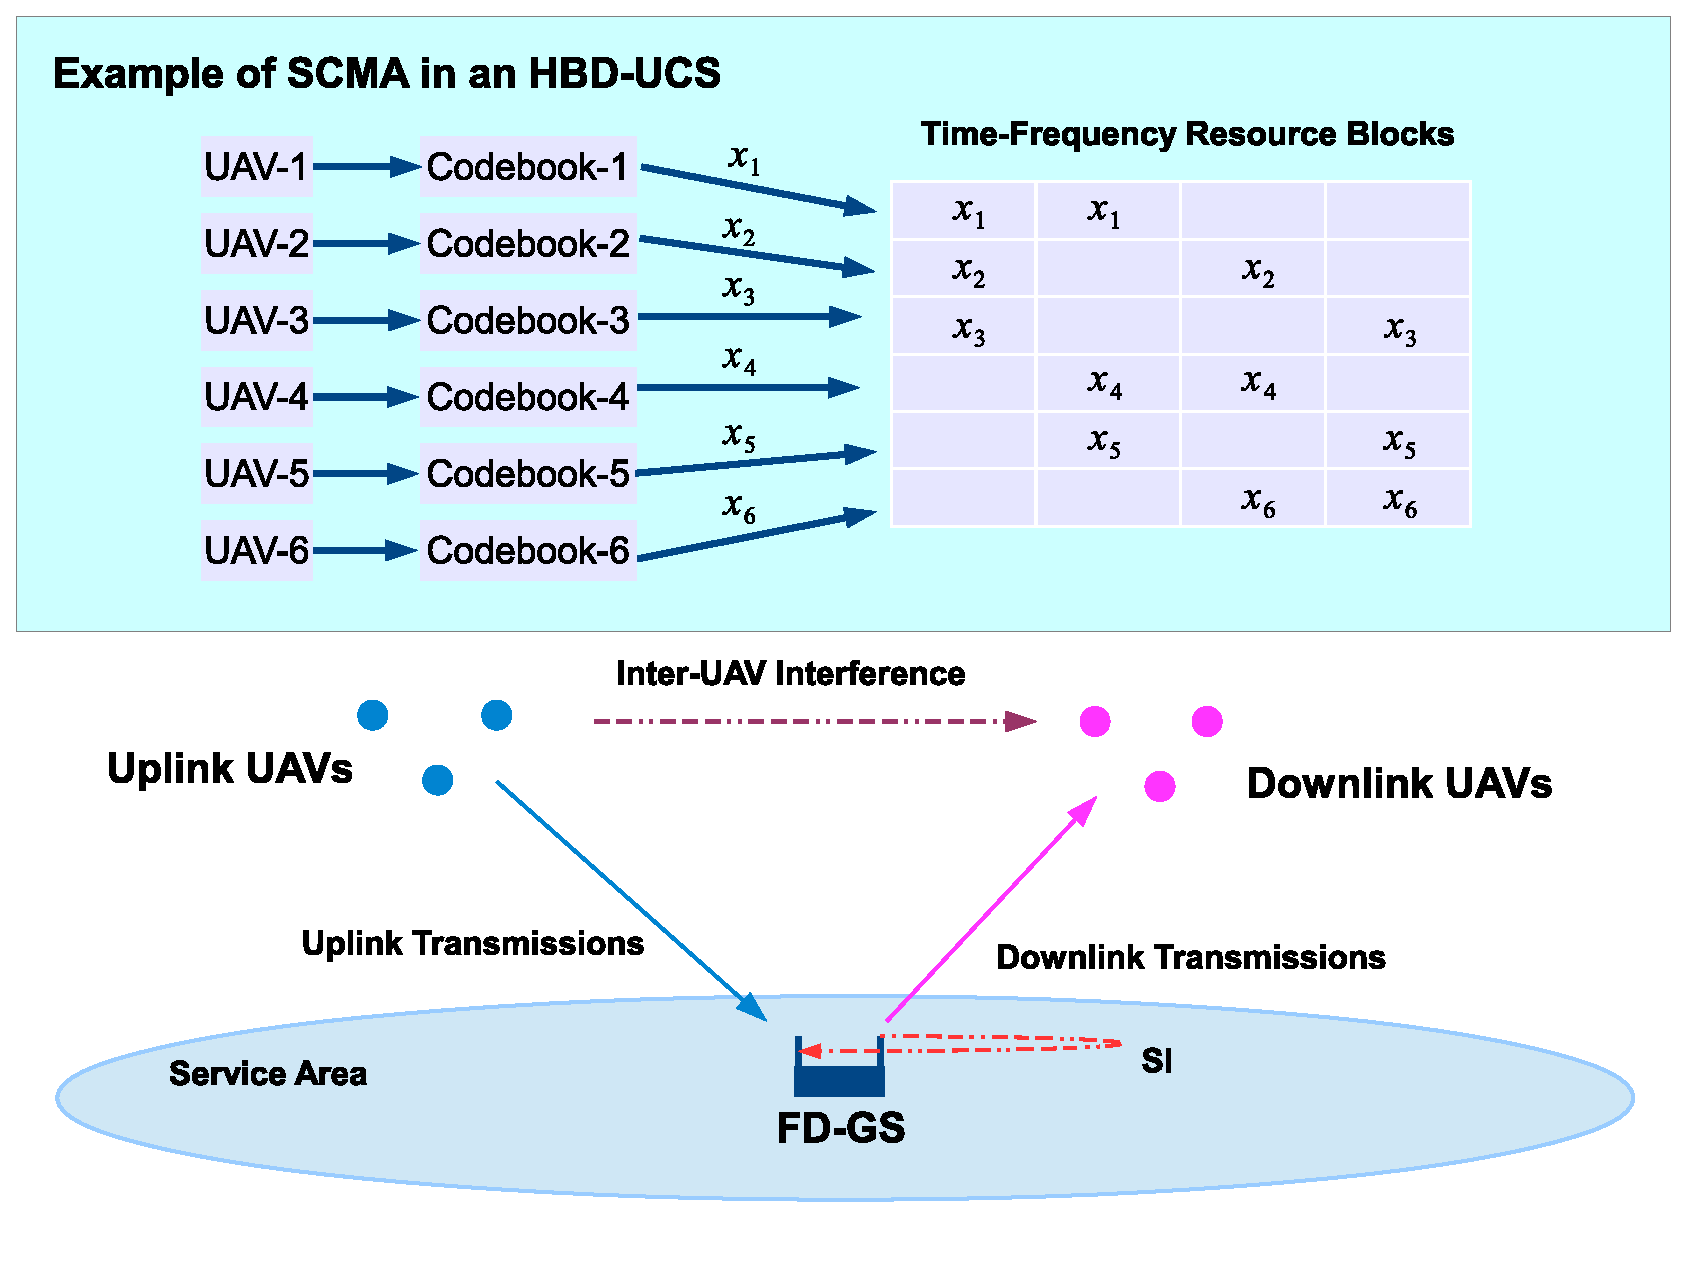
\includegraphics [width=0.6\columnwidth]{chap2_fig/SCMA_HBD_UCS_example.eps} 
%\vspace{-1.5cm}
\caption{An example of implementing SCMA in an HBD-UCS for 3 uplink UAVs (UAV-1, UAV-2, UAV-3) and 3 downlink UAVs (UAV-4, UAV-5, UAV-6) over 4 time-frequency resource blocks. The variable $x_i$ represents the desired message of UAV-$i$.}
%\vspace{-0.5cm}
\label{fig:lit_review_SCMA_HBD_UCS_example}
\end{figure}

In code-domain NOMA, spreading sequences are employed to enable users in the network to share the same time-frequency resource. Although similar in principle to CDMA, the main differentiating factor of code-domain NOMA lies in the fact that only sparse sequences or non-orthogonal low cross correlation sequences are employed to distinguish users \cite{islam2017power,dai2018survey}. Dominant techniques in code-domain NOMA include low-density spreading (LDS) CDMA, i.e., LDS-CDMA \cite{hoshyar2008novel,razavi2011information,islam2017power,dai2018survey}, LDS-based orthogonal frequency-division multiplexing (LDS-OFDM) \cite{hoshyar2010lds,al2014uplink,islam2017power,dai2018survey}, and sparse code multiple access (SCMA) \cite{islam2017power,dai2018survey,nikopour2013sparse,mu2015fixed,du2016fast}. In LDS-CDMA, the symbols of each user are mapped to an LDS sequence before transmission \cite{dai2018survey,hoshyar2008novel}. User detection is then performed on the received composite signal by employing the sum-product algorithm used in low-density parity-check decoding \cite{hoshyar2008novel}. For LDS-OFDM, user symbols are mapped to LDS sequences before transmission over a set of subcarriers \cite{islam2017power,dai2018survey}. In contrast to LDS-CDMA and LDS-OFDM, SCMA employs bit-to-constellation mapping and spreading operations to generate unique codewords for each user \cite{islam2017power,dai2018survey,nikopour2013sparse}. An example of SCMA in an HBD-UCS is depicted in Fig. \ref{fig:lit_review_SCMA_HBD_UCS_example} for 3 uplink UAVs (UAV-1, UAV-2, UAV-3) and 3 downlink UAVs (UAV-4, UAV-5, UAV-6) over 4 time-frequency resource blocks. Specifically, the uplink UAVs employ codebook-$i, 1 \leq i \leq 3$ to transmit the desired message $x_i$ to the FD-GS. Simultaneously, the FD-GS employs codebook-$j, 4 \leq j \leq 6$ to transmit the desired message $x_j$ to the downlink UAVs. Thus, the desired messages of UAV-1, UAV-2, and UAV-3 are multiplexed onto the same time-frequency resource block. Likewise, the desired messages of UAV-1, UAV-4, and UAV-5 are also multiplexed onto the same time-frequency resource block. Although promising, code-domain NOMA techniques achieve spectrum efficiency improvements at the cost of signaling cost and high complexity \cite{dai2018survey}.

\subsubsection{Power-Domain NOMA}

Users in power-domain share the same time-frequency resource in power-domain through superposition coding \cite{islam2017power,dai2018survey,kader2018full,cui2016novel,salehi2019meta,ernest2019noma,liu2018heterogeneous,wang2017sir,kader2018coordinated,zhang2017downlink,ding2016general,ding2016impact,liang2017user}. In particular, for uplink transmissions, users are distinguished through an unequal allocation of transmit powers before signal transmission in power-domain NOMA. Thereafter, all uplink users transmit the intended message to the receiver, e.g., base stations, effectively forming a multiple-access channel. Then, SIC detection is successively employed on the received composite signal to recover the desired messages from all users in the presence of multi-user interference (MUI) \cite{cui2016novel,kader2018full,salehi2019meta,weber2007transmission,islam2017power}. For downlink transmissions in power-domain NOMA, the transmitter, e.g., a base station, similarly distinguishes downlink users through an unequal allocation of transmit powers \cite{islam2017power}. The transmitter then superimposes all intended messages into a composite signal before transmitting it to the downlink users, thus forming a broadcast channel. Under such a scenario, MUI is experienced by the downlink users. For downlink users experiencing strong MUI, SIC detection is successively employed until the desired message is recovered. On the other hand, II detection is employed at downlink users with weak MUI. For cases where MUI is neither weak nor strong, partial interference cancellation is employed to cancel MUI signals that are stronger than the desired message \cite{salehi2019meta,islam2017power}.

\begin{figure} [t]
\centering
%\vspace{-1.5cm}
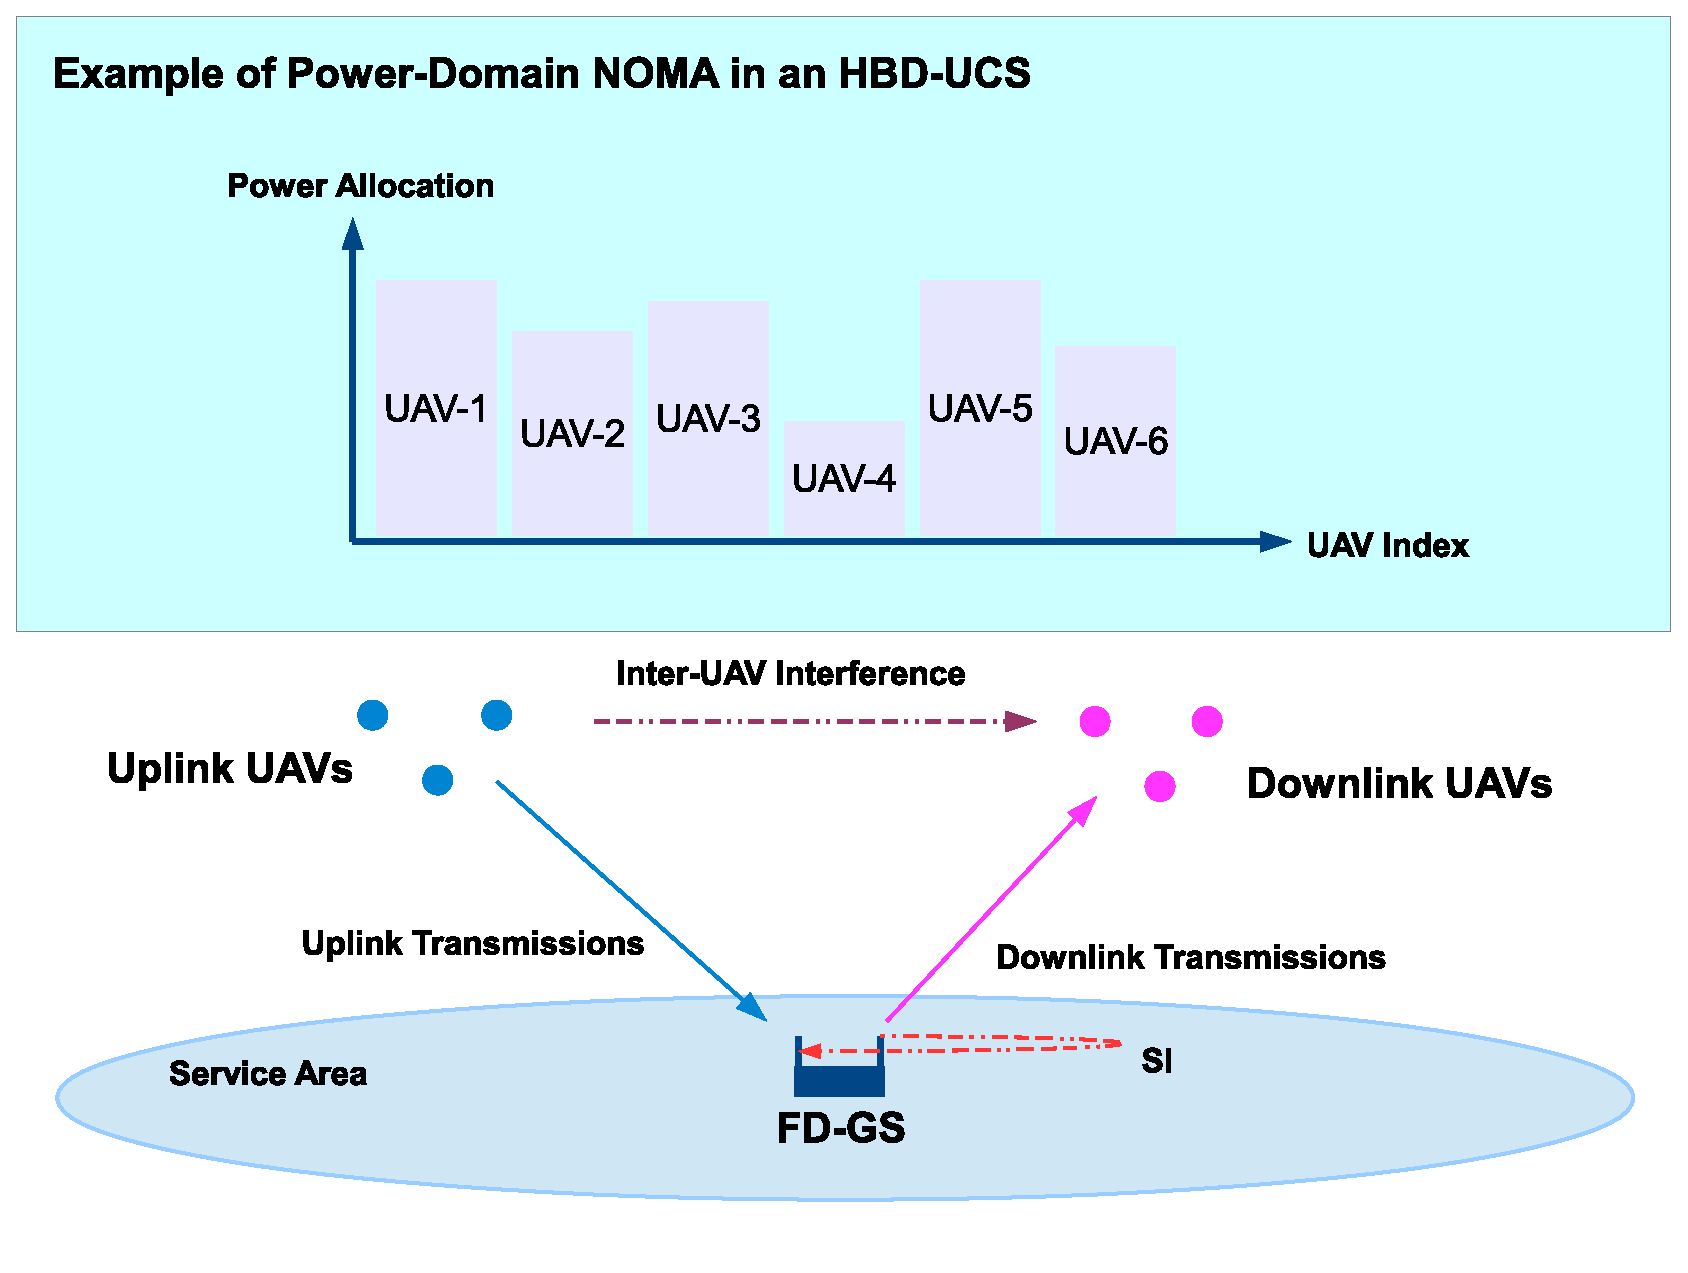
\includegraphics [width=0.6\columnwidth]{chap2_fig/power_domain_NOMA_HBD_UCS_example.eps} 
%\vspace{-1.5cm}
\caption{An example of implementing power-domain NOMA in an HBD-UCS for 3 uplink UAVs (UAV-1, UAV-2, UAV-3) and 3 downlink UAVs (UAV-4, UAV-5, UAV-6) over the same time-frequency resource block.}
%\vspace{-0.5cm}
\label{fig:lit_review_power_domain_NOMA_HBD_UCS_example}
\end{figure}


\subsubsection{Relevance of Power-Domain NOMA in an HBD-UCS}

From the above discussions, transmit power allocation and SIC error propagation are some of the practical considerations of power-domain NOMA \cite{islam2017power,dai2018survey}. However, power-domain NOMA enables the number of users sharing the same time-frequency resource to be easily scalable. Furthermore, compared to conventional OMA schemes, power-domain NOMA can offer higher spectrum efficiency and is also capable of achieving the capacity region of broadcast channels \cite{dai2018survey}.\footnote{We refer to frequency division multiple access (FDMA), TDMA, and CDMA as conventional OMA schemes in this survey.}

In the context of HBD UAV communications, power-domain NOMA is a suitable technique to enable multi-UAV deployment in HBD UAV communications. To illustrate this point, recall that the system model in Fig. \ref{fig:lit_review_interference_management_example} assumes only one uplink UAV and one downlink UAV concurrently communicating on the same spectrum. Such an assumption may not be realistic as arbitrary numbers of uplink and downlink UAVs can be simultaneously deployed in the HBD-UCS. To this end, the system model in Fig. \ref{fig:lit_review_interference_management_example} and the resultant signal models at the FD-enabled GS and downlink UAVs can be easily extended to account for arbitrary numbers of uplink and downlink UAVs, with an example illustrated in Fig. \ref{fig:lit_review_power_domain_NOMA_HBD_UCS_example}. However, doing so introduces MUI at both the FD-enabled GS and downlink UAVs, and uplink interference, i.e., inter-UAV interference, at the downlink UAVs \cite{ernest2019noma}. Thus, a multi-UAV deployment scenario naturally raises questions on how the detection process at the FD-enabled GS and downlink UAVs can be conducted in the presence of MUI and uplink interference. In this aspect, power-domain NOMA can be employed in an HBD-UCS for multi-UAV deployment scenarios. For instance, at the FD-enabled GS, SIC detection can be employed to recover messages from the uplink UAVs in the presence of MUI. For the downlink UAVs, SIC and II detection can be employed to recover the desired message from the FD-enabled GS while mitigating MUI and inter-UAV interference from the uplink UAVs.

With the above reasons in mind, the feasibility of power-domain NOMA for HBD UAV communications will be studied in the later part of this thesis.

%%%%%%%%%%%%%%%%%%%%%%%%%%%%%%%%%%%%%%%%%%%%%%%%%%%%%%%%%%%%%%%%%%%%%%%%%%%%%%%%%%%%%%%%%%%%%%%%%%%%%%%%%%%%%%%%%%%%%%%%%%%%%%%%%%%%%%%%%
% Section: Conclusion
\section{Chapter Summary} \label{lit_review_sec_conclusion}

In this chapter, we reviewed vital enabling techniques in realizing HBD UAV communications to improve spectrum efficiency. First, a review of recent advances in UAV channel modeling for HBD UAV communications was presented\textcolor{black}{, where it was shown that UAV channels can be modeled using common fading models such as Rician fading}. The types of SI mitigation architectures that can be implemented at FD-enabled GSs were also surveyed. \textcolor{black}{It was also noted that phase noise, SI channel estimation errors, and quantization noise are the main sources of residual SI for FD transceivers}. For the HD UAVs, a survey of interference management techniques, which focuses on II, SIC, and JD strategies, was conducted to address inter-UAV interference. Apart from discussing the state-of-the-art, the performance of II, SIC, and JD approaches were discussed in terms of outage probability and finite SNR diversity gain. \textcolor{black}{For multi-UAV HBD-UCSs, an overview of NOMA techniques was discussed to support multi-UAV deployment. The suitability of power-domain NOMA for multi-UAV networks highlighted, although the feasibility of power-domain NOMA for multi-UAV networks remains an open research problem.}




